\begin{figure}[!t]
  % \hspace{1.5cm}
\center
% \begin{tabular}{c|c|c|c}
\definecolor{darkgreen}{rgb}{0, 0.5, 0}
\newcommand{\bluetri}{{\color{blue} $\blacktriangle$}}
\newcommand{\greentri}{{\color{darkgreen} $\blacktriangle$}}
\newcommand{\redtri}{{\color{red} $\blacktriangle$}}
\newcommand{\bluecir}{{\color{blue} $\circ$}}
\newcommand{\greencir}{{\color{darkgreen} $\circ$}}
\newcommand{\redcir}{{\color{red} $\circ$}}
\begin{tabular}{cc}
\panel{A} & \hspace{-1cm}\panel{B} \\[-.7cm]
% \raisebox{8.7cm}{\hspace{-0.2cm}} %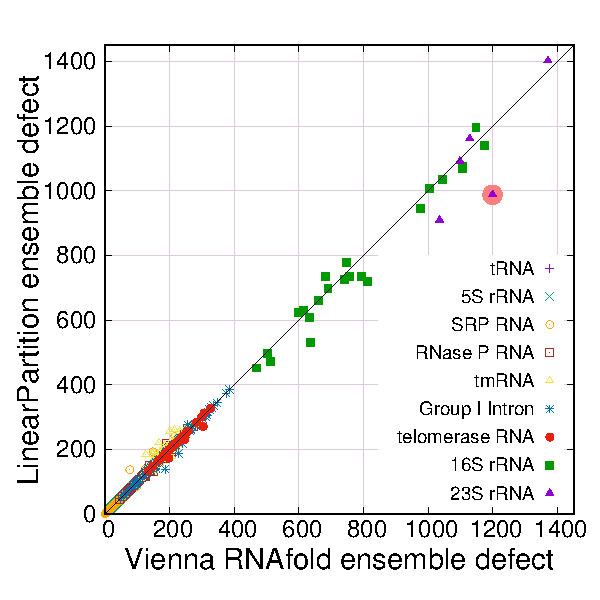
\includegraphics[width=0.4\textwidth]{figs/ensemble_defect} }
% &
% \hspace{-.2cm}\panel{A} & \hspace{-0.6cm}\panel{B} \\[-1cm] %& \hspace{-2.5cm}\panel{D}
	\multicolumn{2}{c}{
	  \hspace{-.3cm}
%          \vspace{-.2cm}
	  \raisebox{7.5cm}
	  {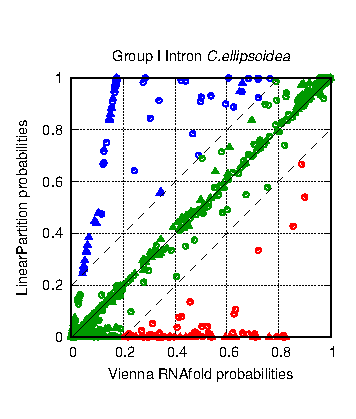
\includegraphics[width=4.4cm]{figs/prob_xy_grp1}}
	  \hspace{-4.5cm}
	   %\raisebox{0cm}
	  {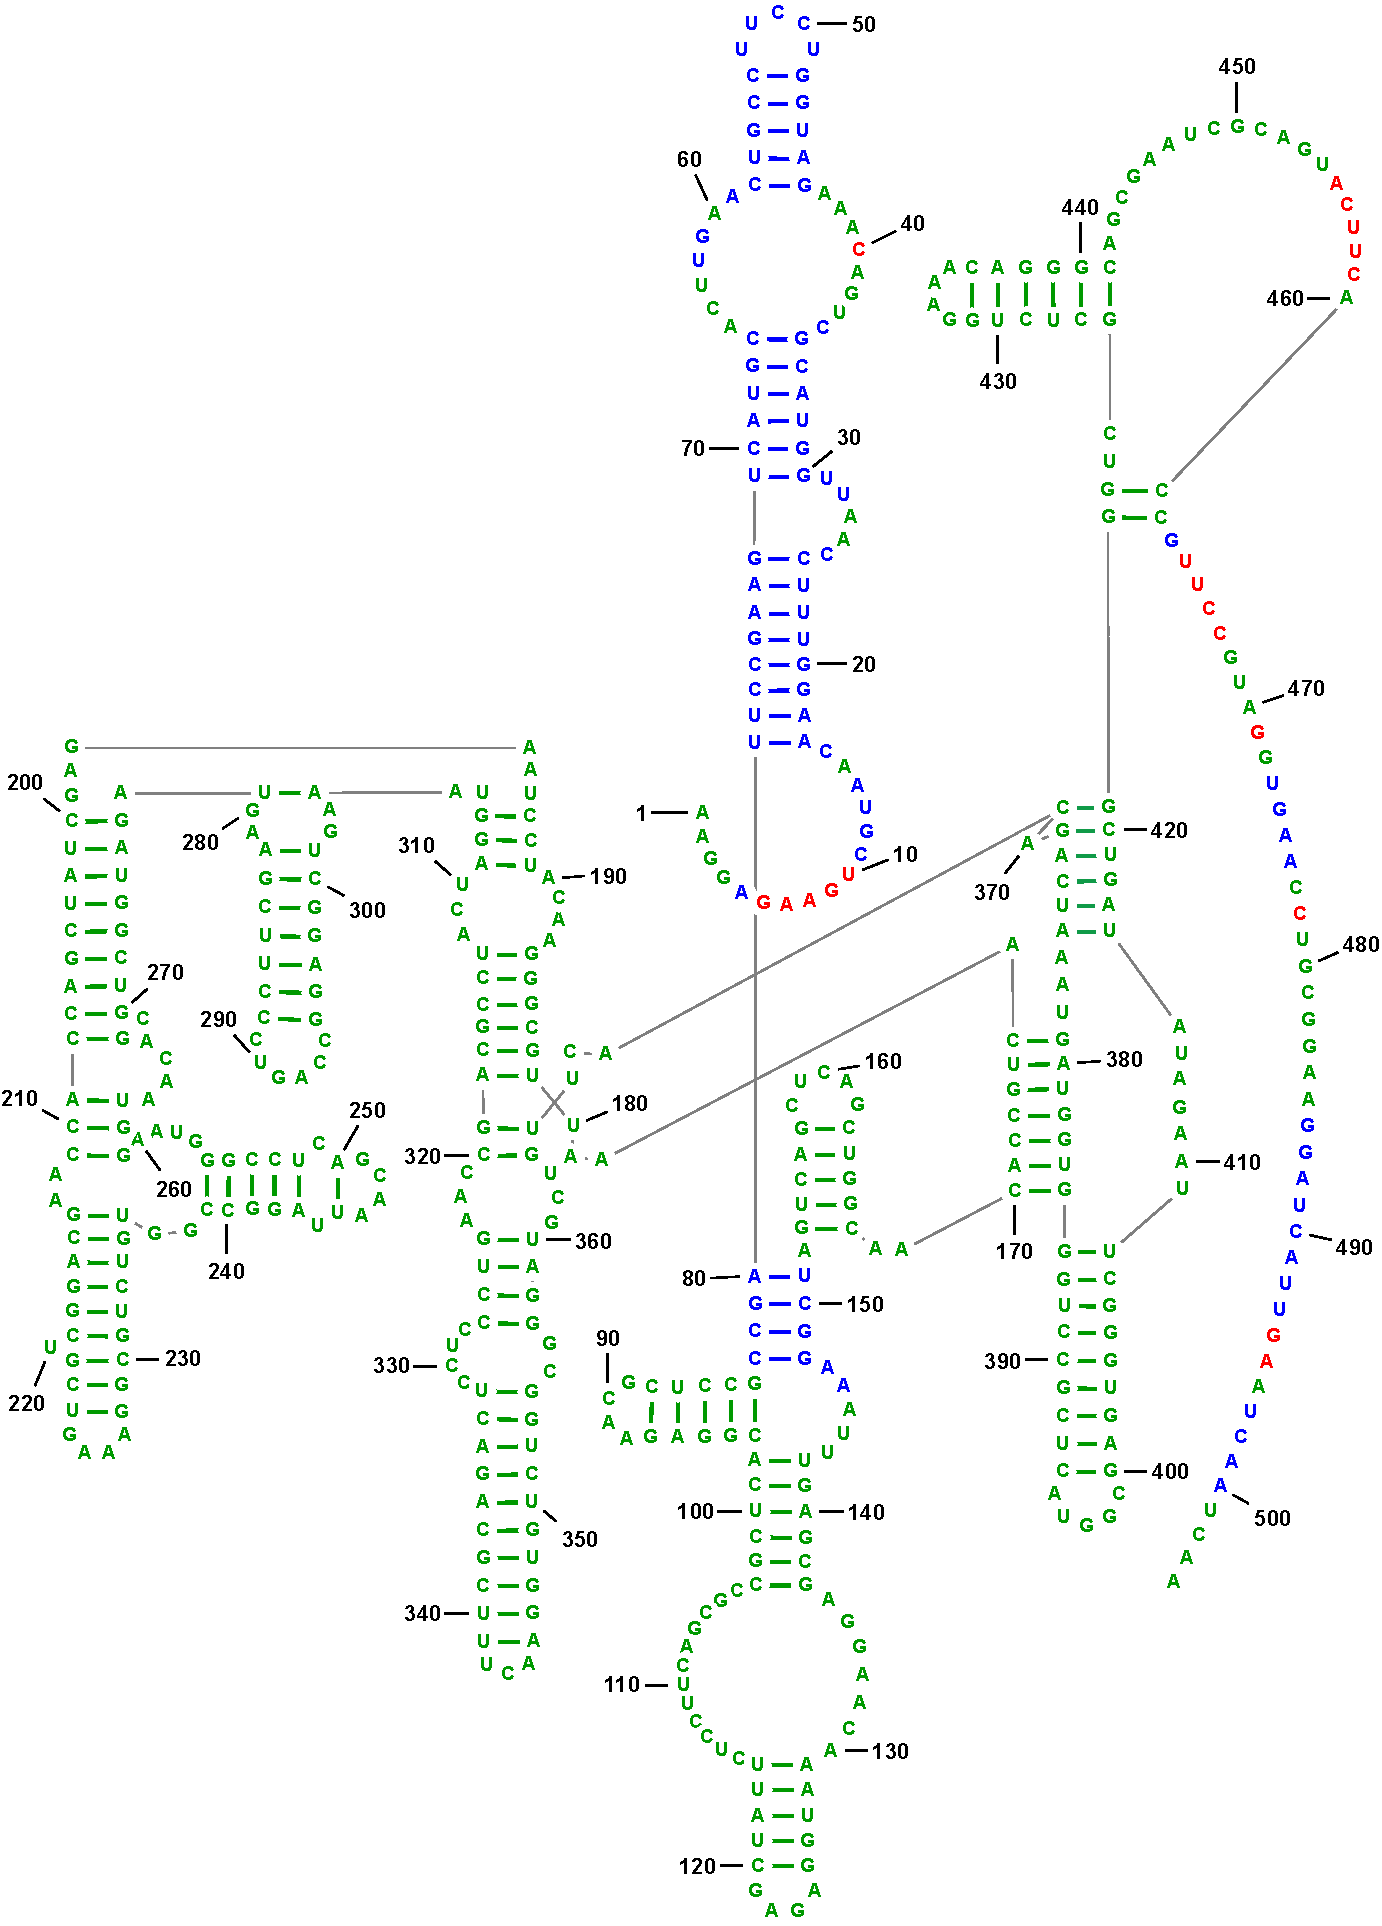
\includegraphics[width=0.5\textwidth]{figs/grp1_70_gutell_modified_2020}}
  	} \\[-1.6cm]
  	\hspace{-.0cm}\panel{C} &  \\[-1.cm]
  	\end{tabular}
% \hspace{-7cm}\panel{B} &\\[-.8cm]

% &&\raisebox{0cm}{\hspace{0.2cm}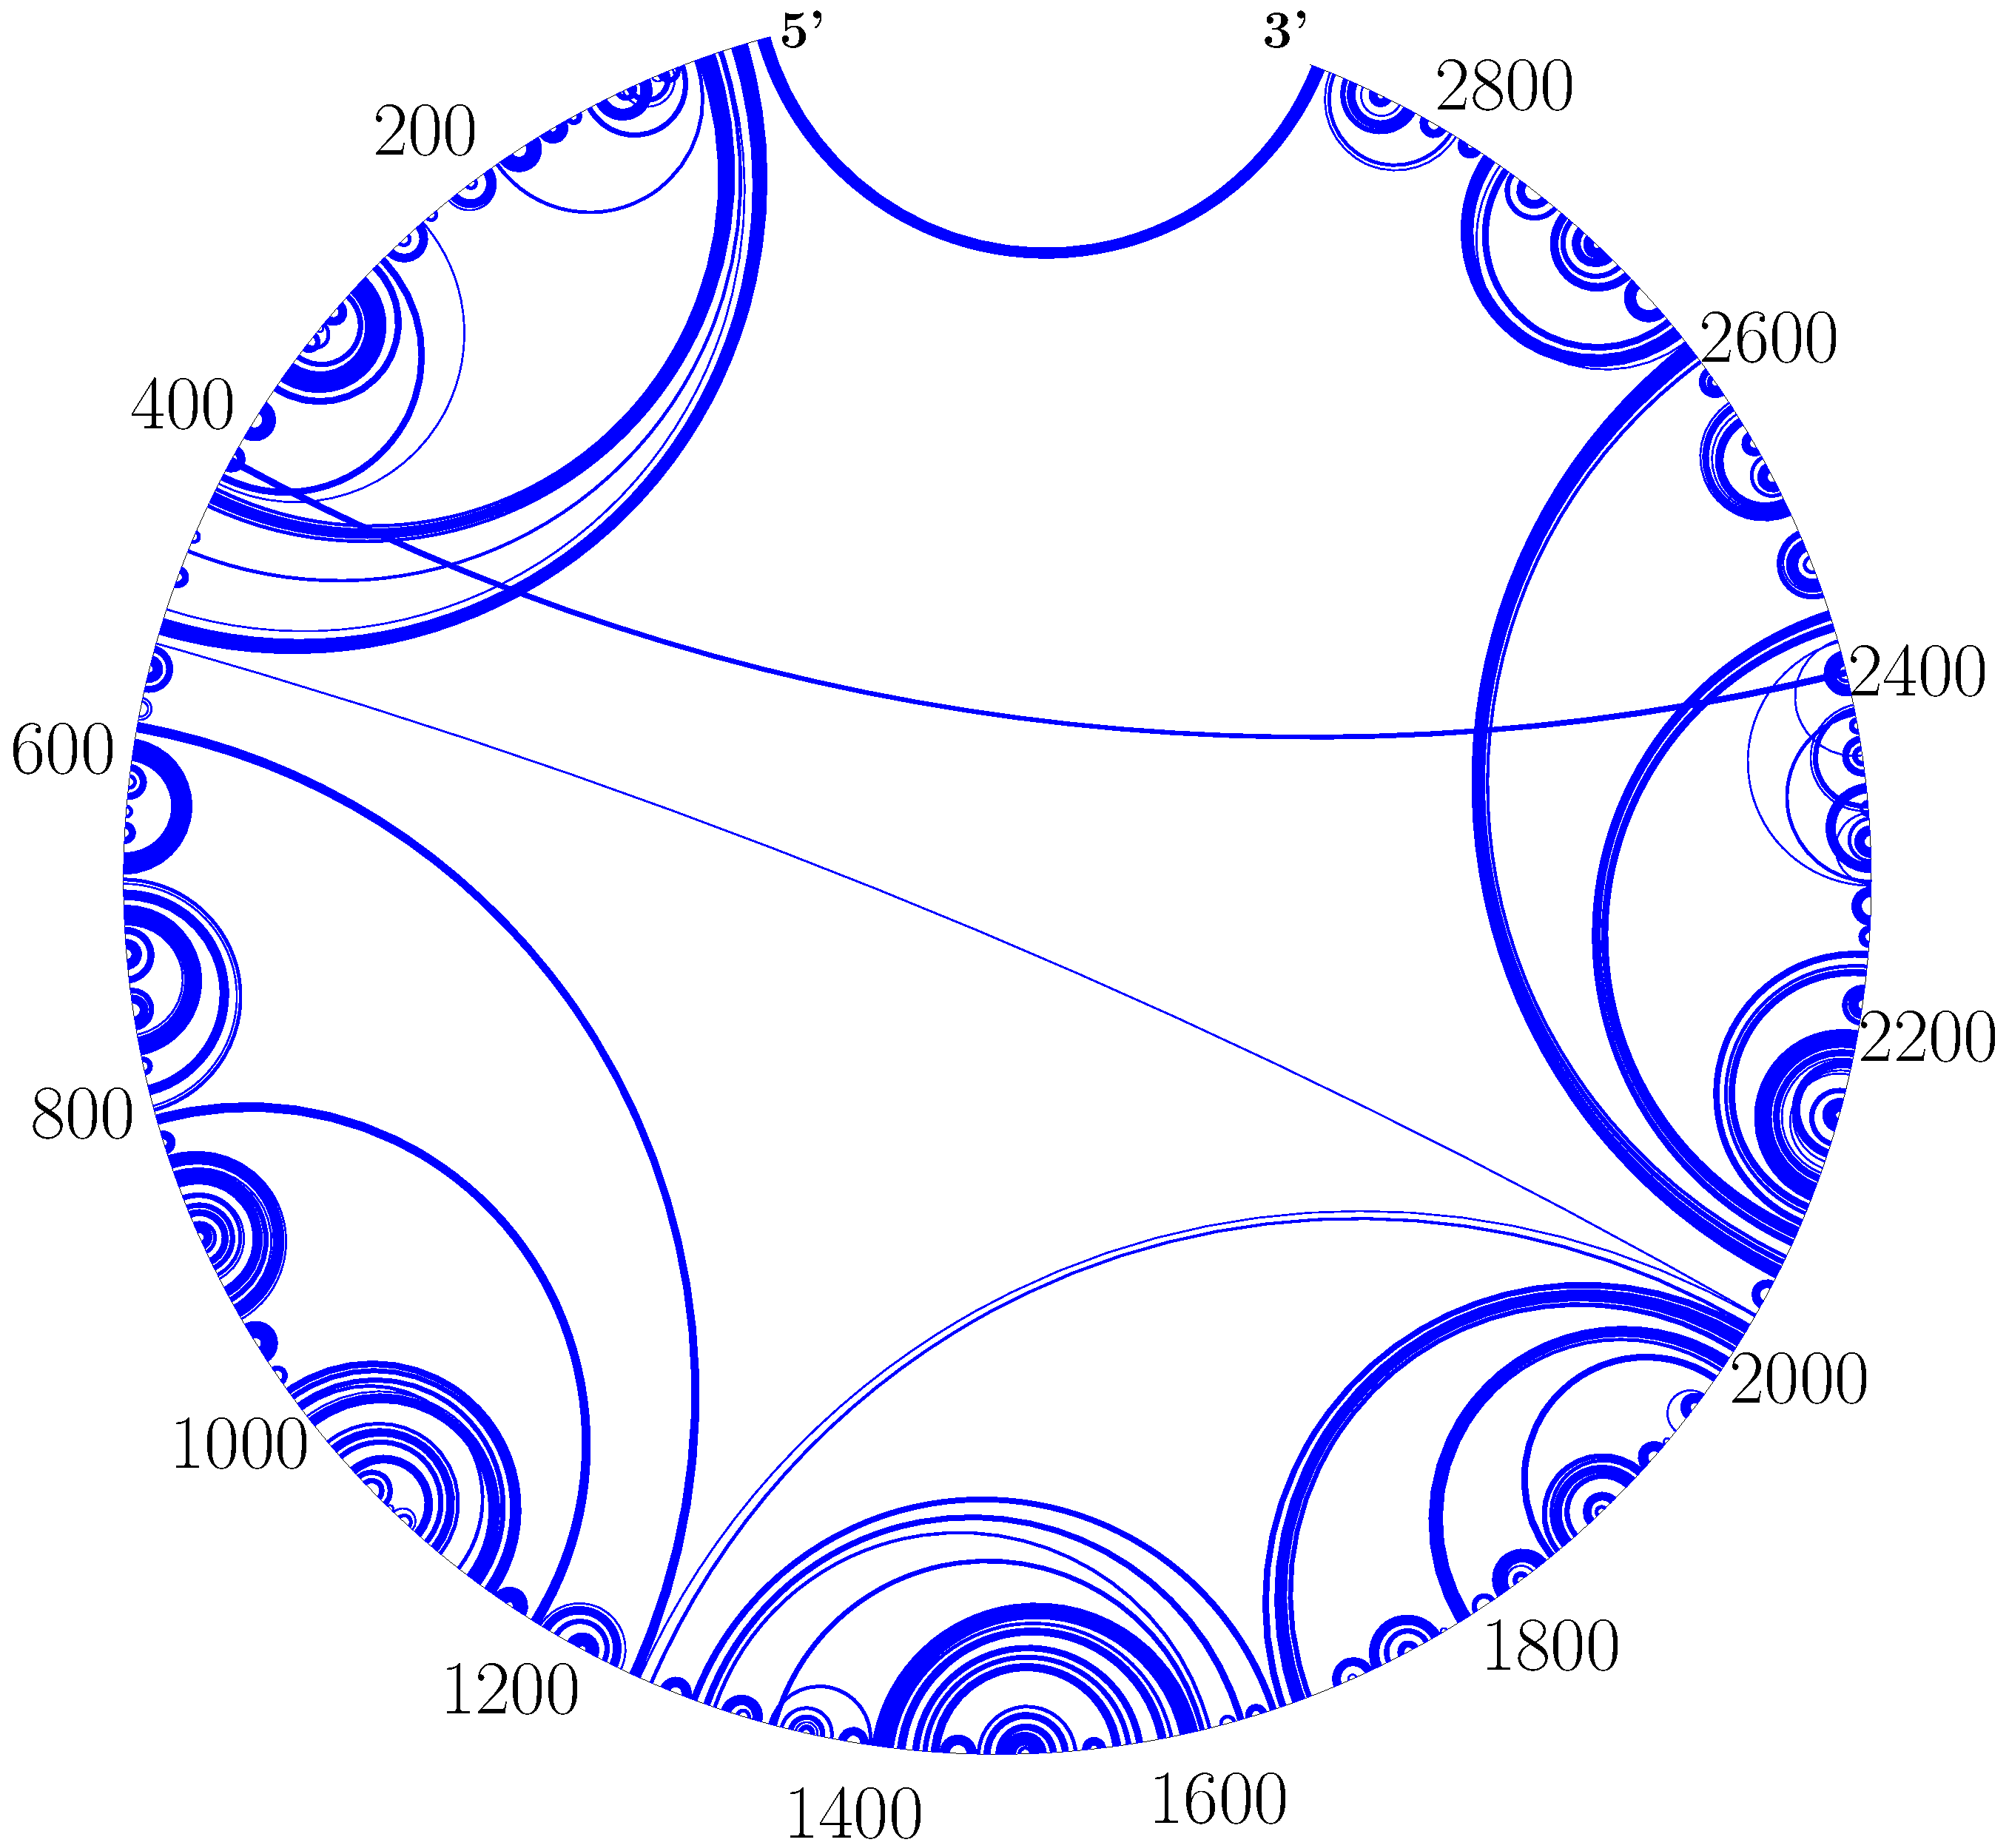
\includegraphics[width=0.25\textwidth]{figs/23s_gold}} \\
% &&\hspace{-4.5cm}\panel{E}\\[-.3cm]
% &&\raisebox{0cm}{\hspace{0.2cm}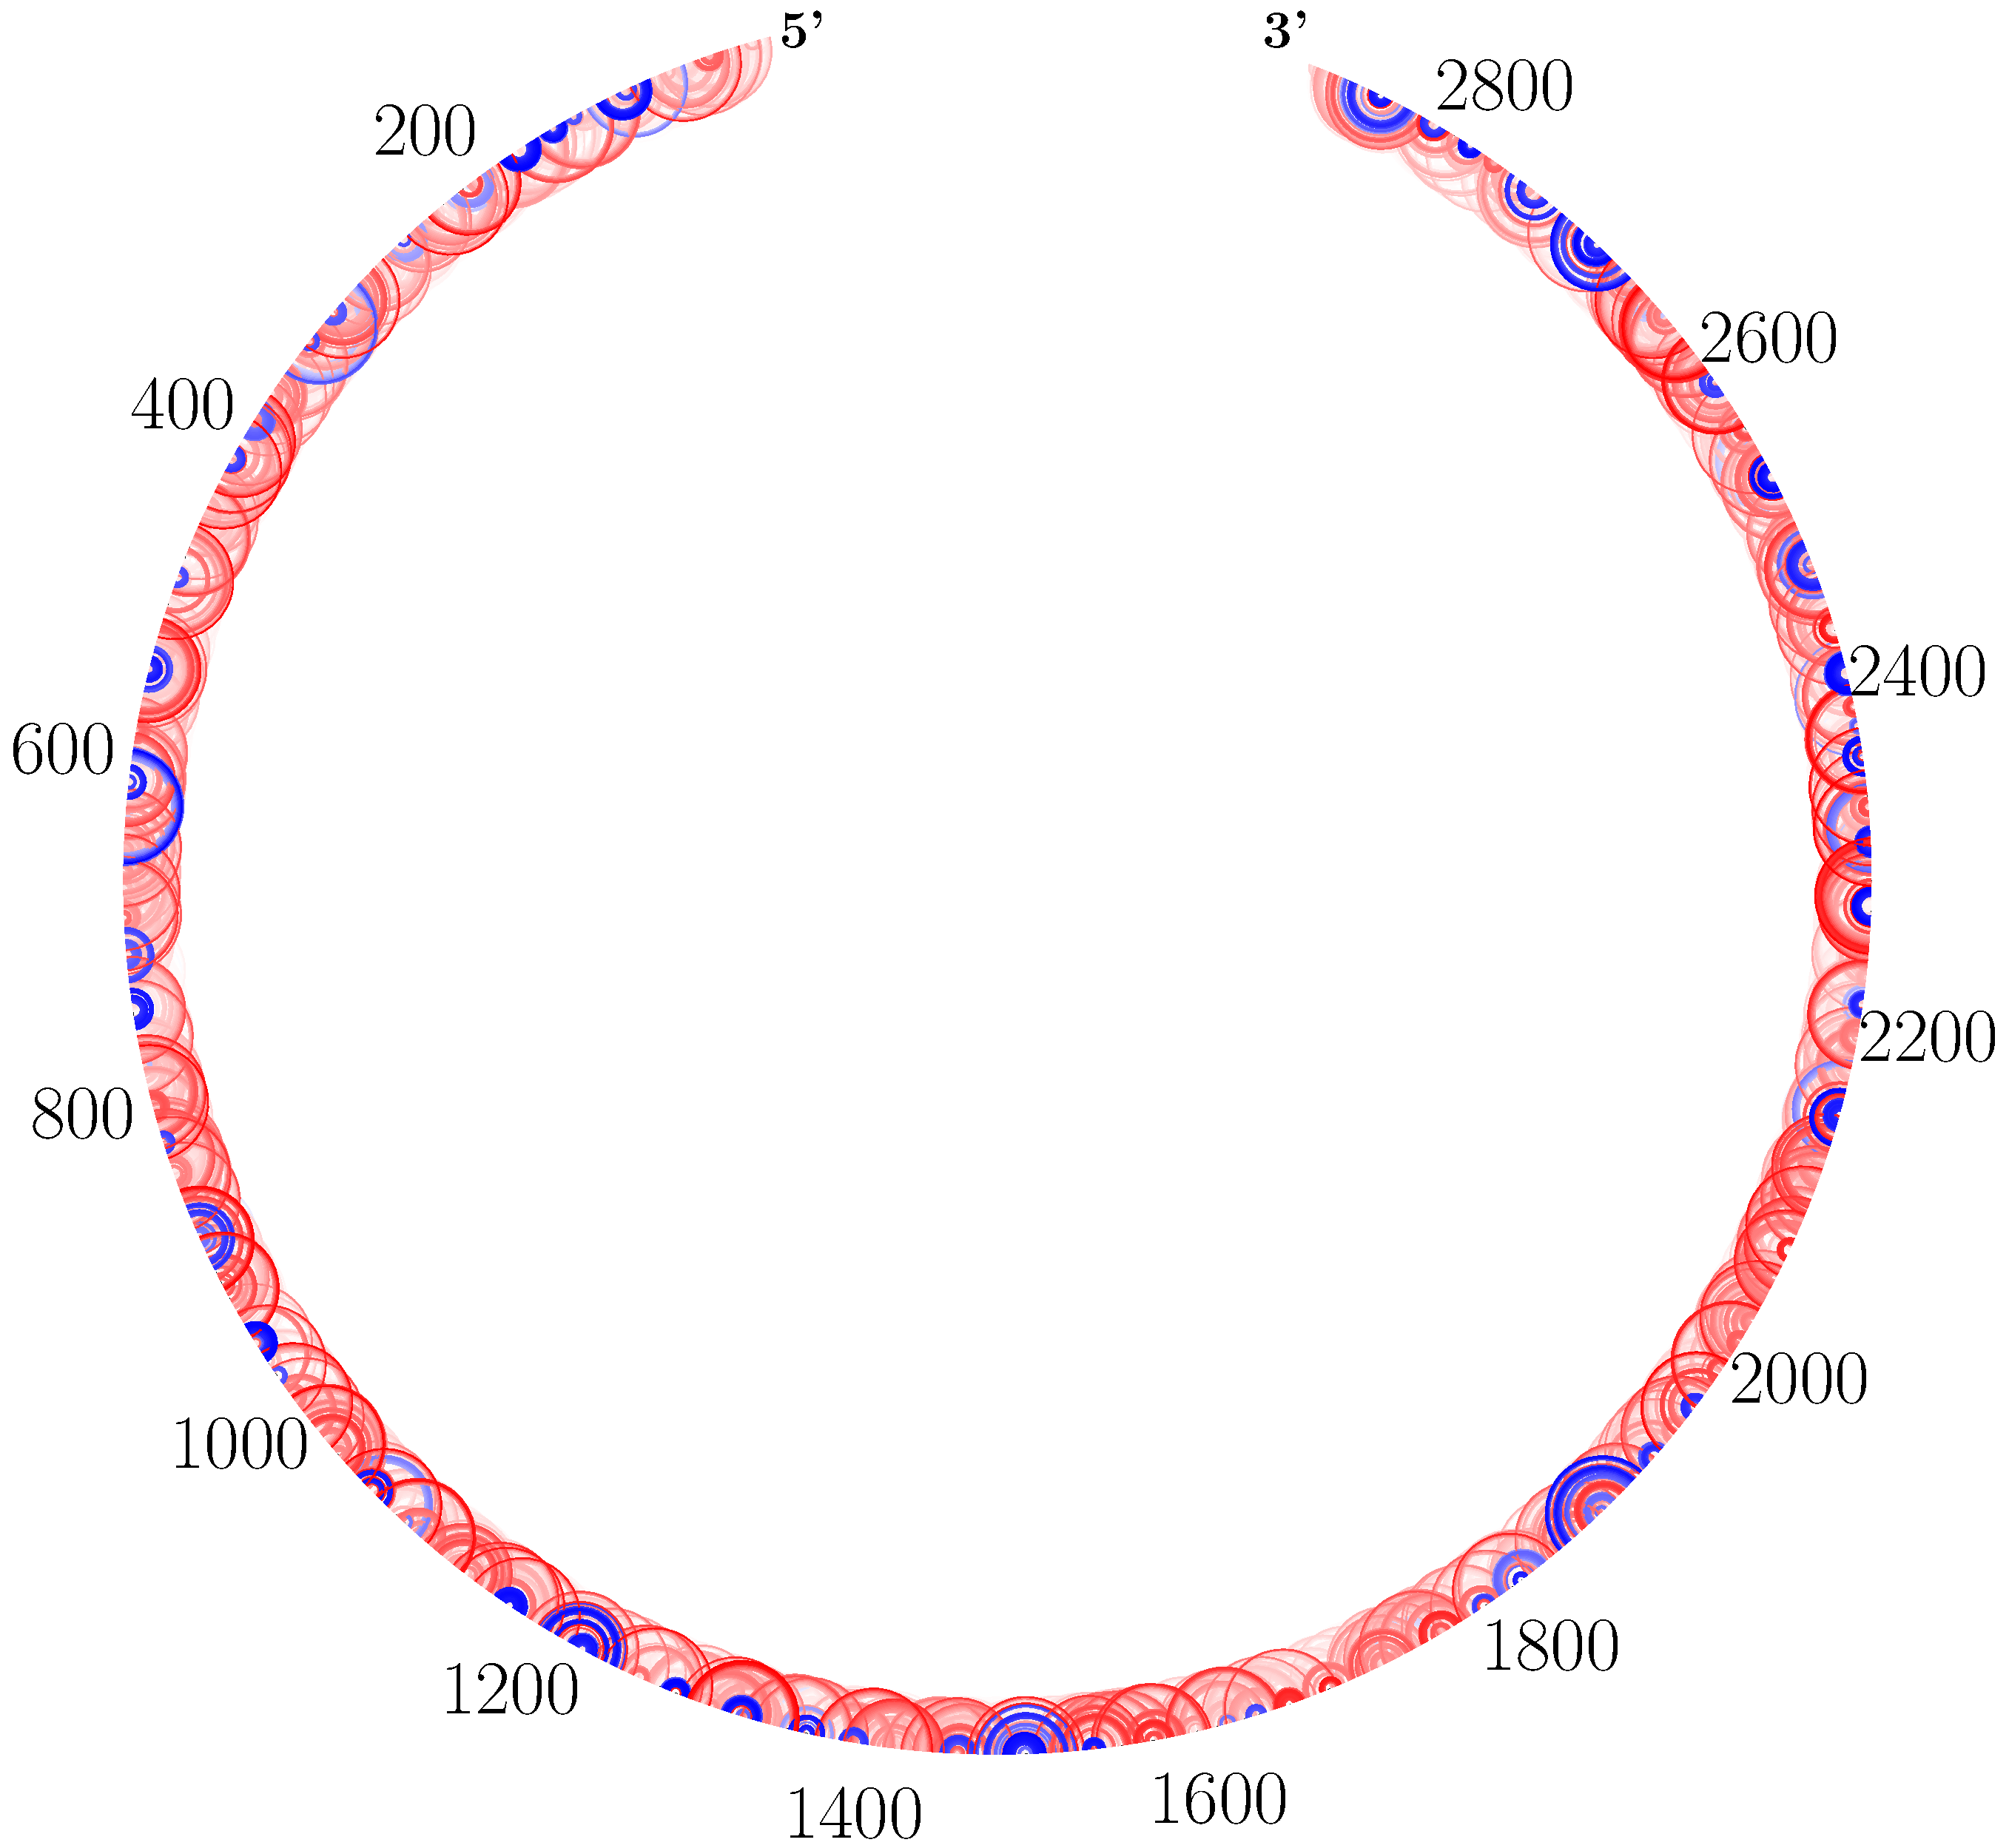
\includegraphics[width=0.25\textwidth]{figs/23s_vienna_plfold_example}} \\
% &&\hspace{-4.5cm}\panel{F}\\[-.3cm]
% &&\raisebox{0cm}{\hspace{0.2cm}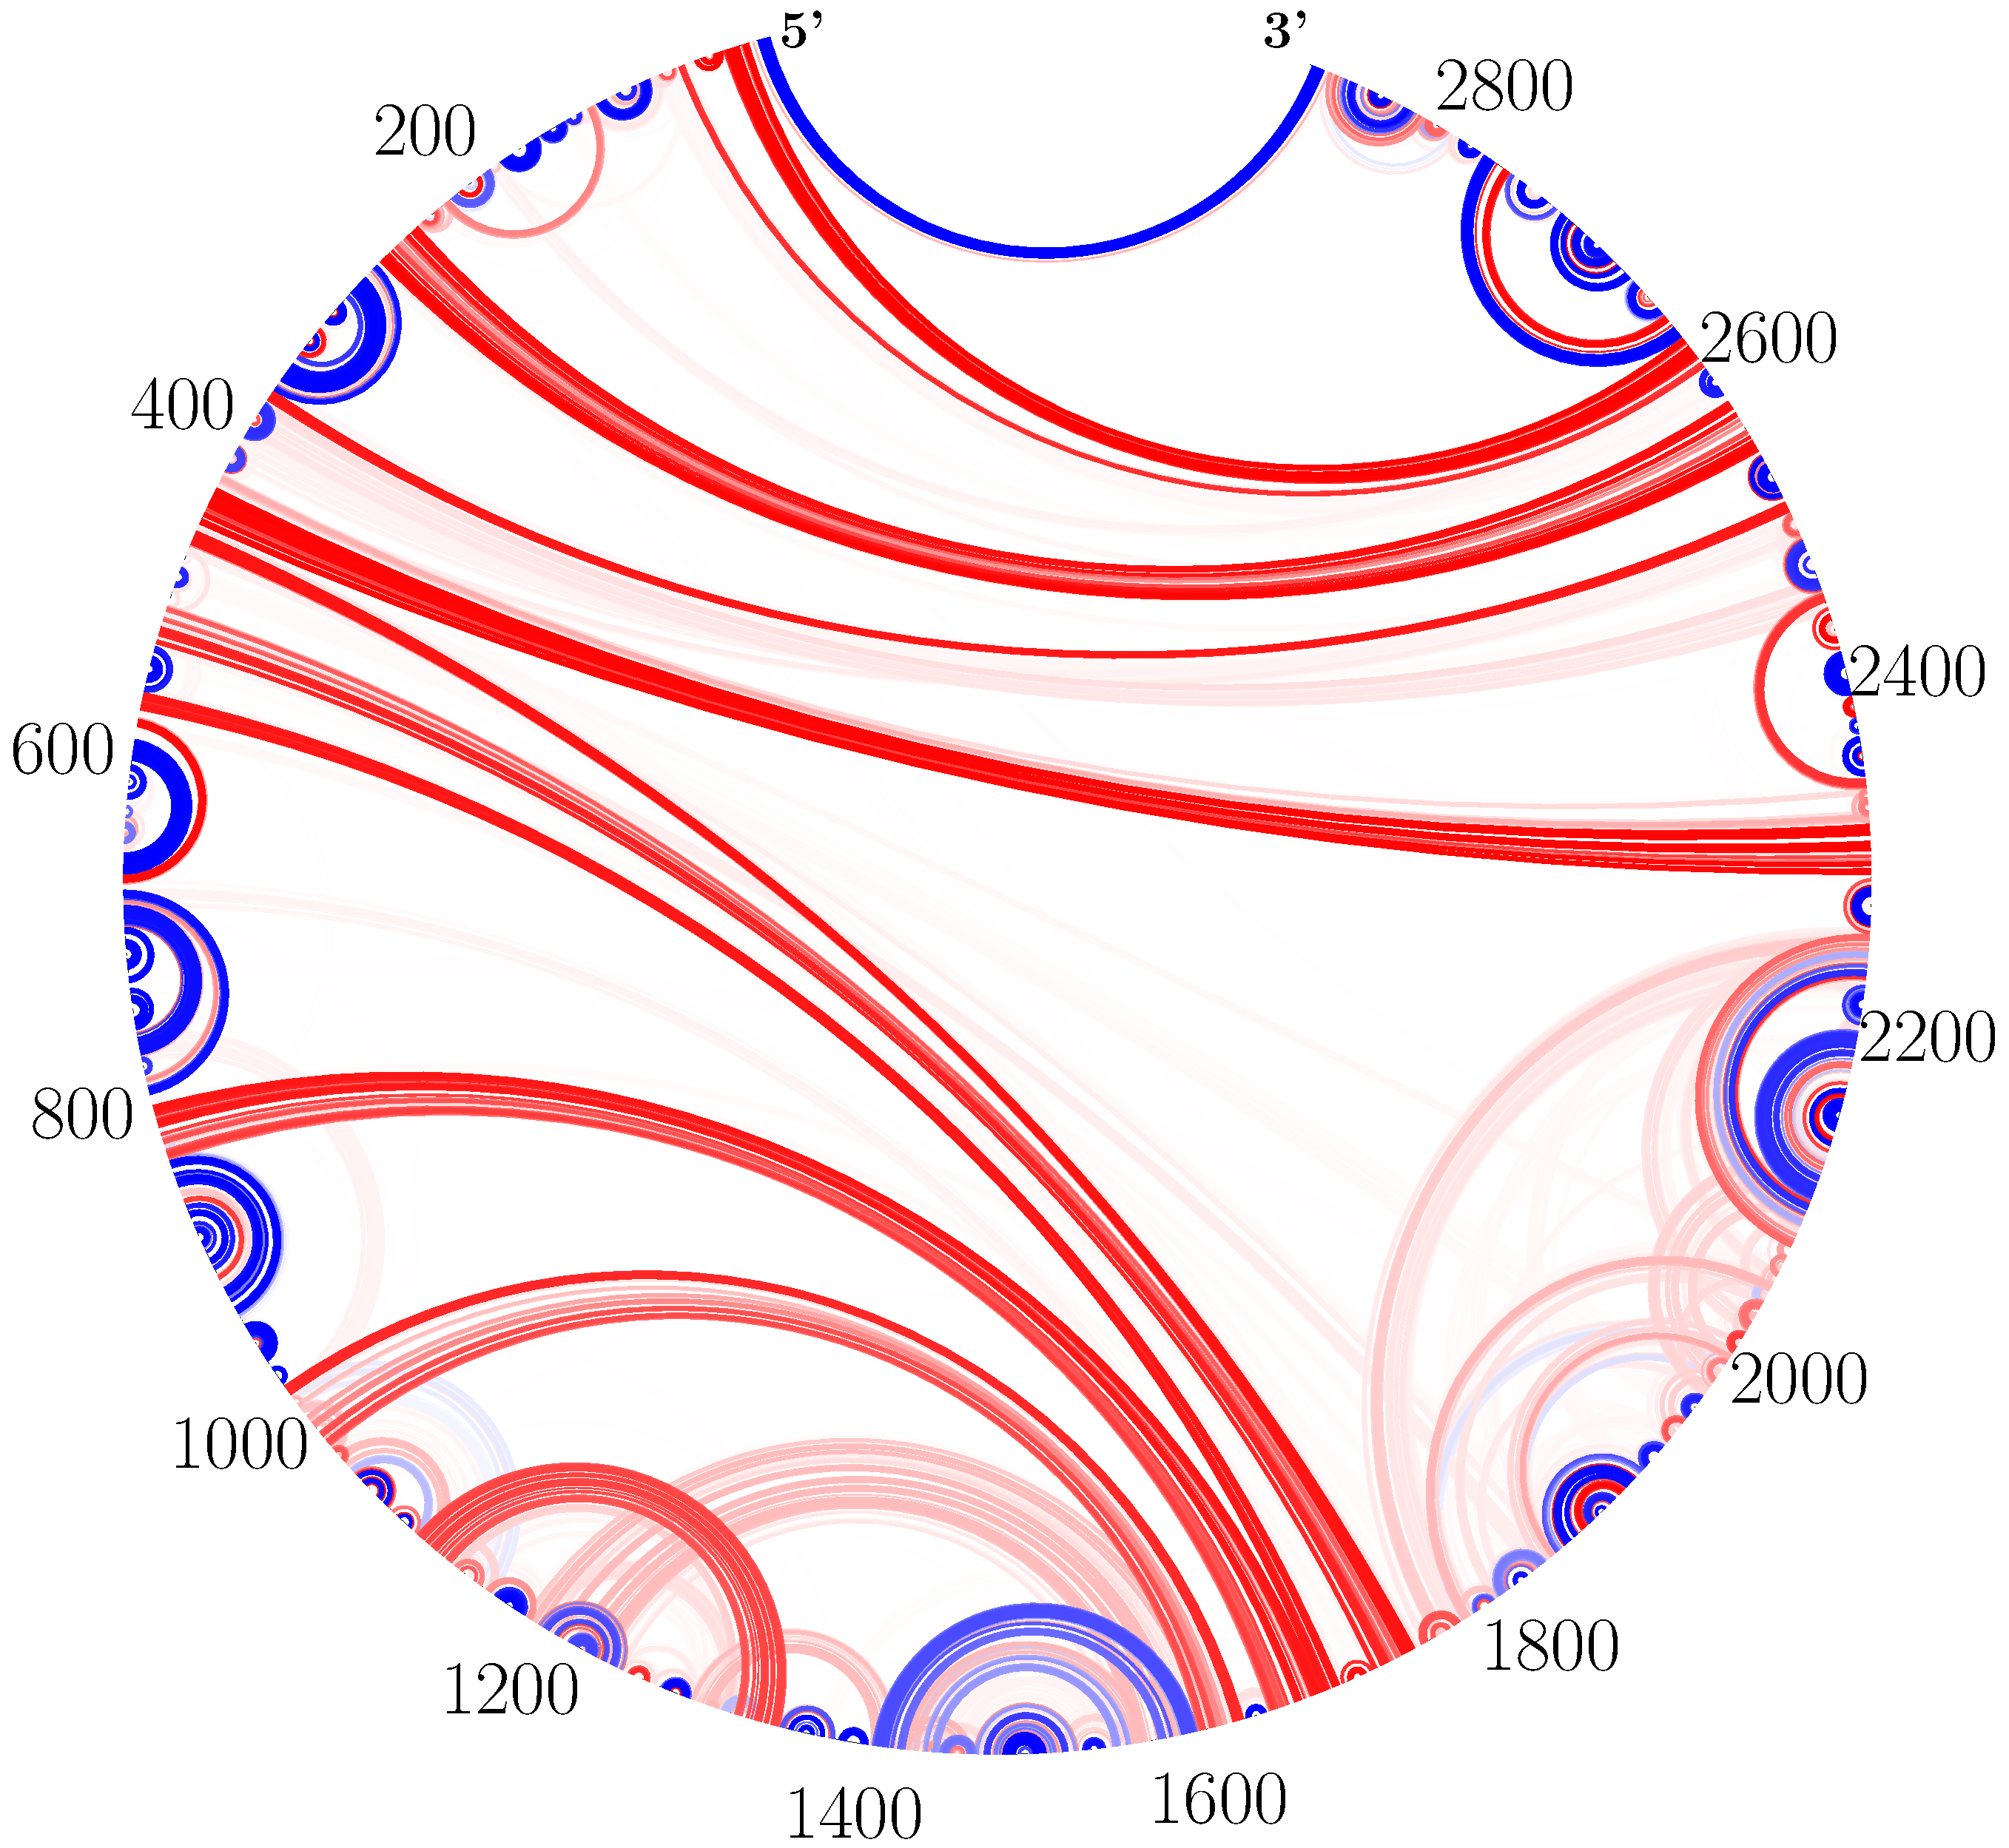
\includegraphics[width=0.25\textwidth]{figs/23s_vienna_example}} \\
% &&\hspace{-4.5cm}\panel{G}\\[-.3cm]
% &&\raisebox{0cm}{\hspace{0.2cm}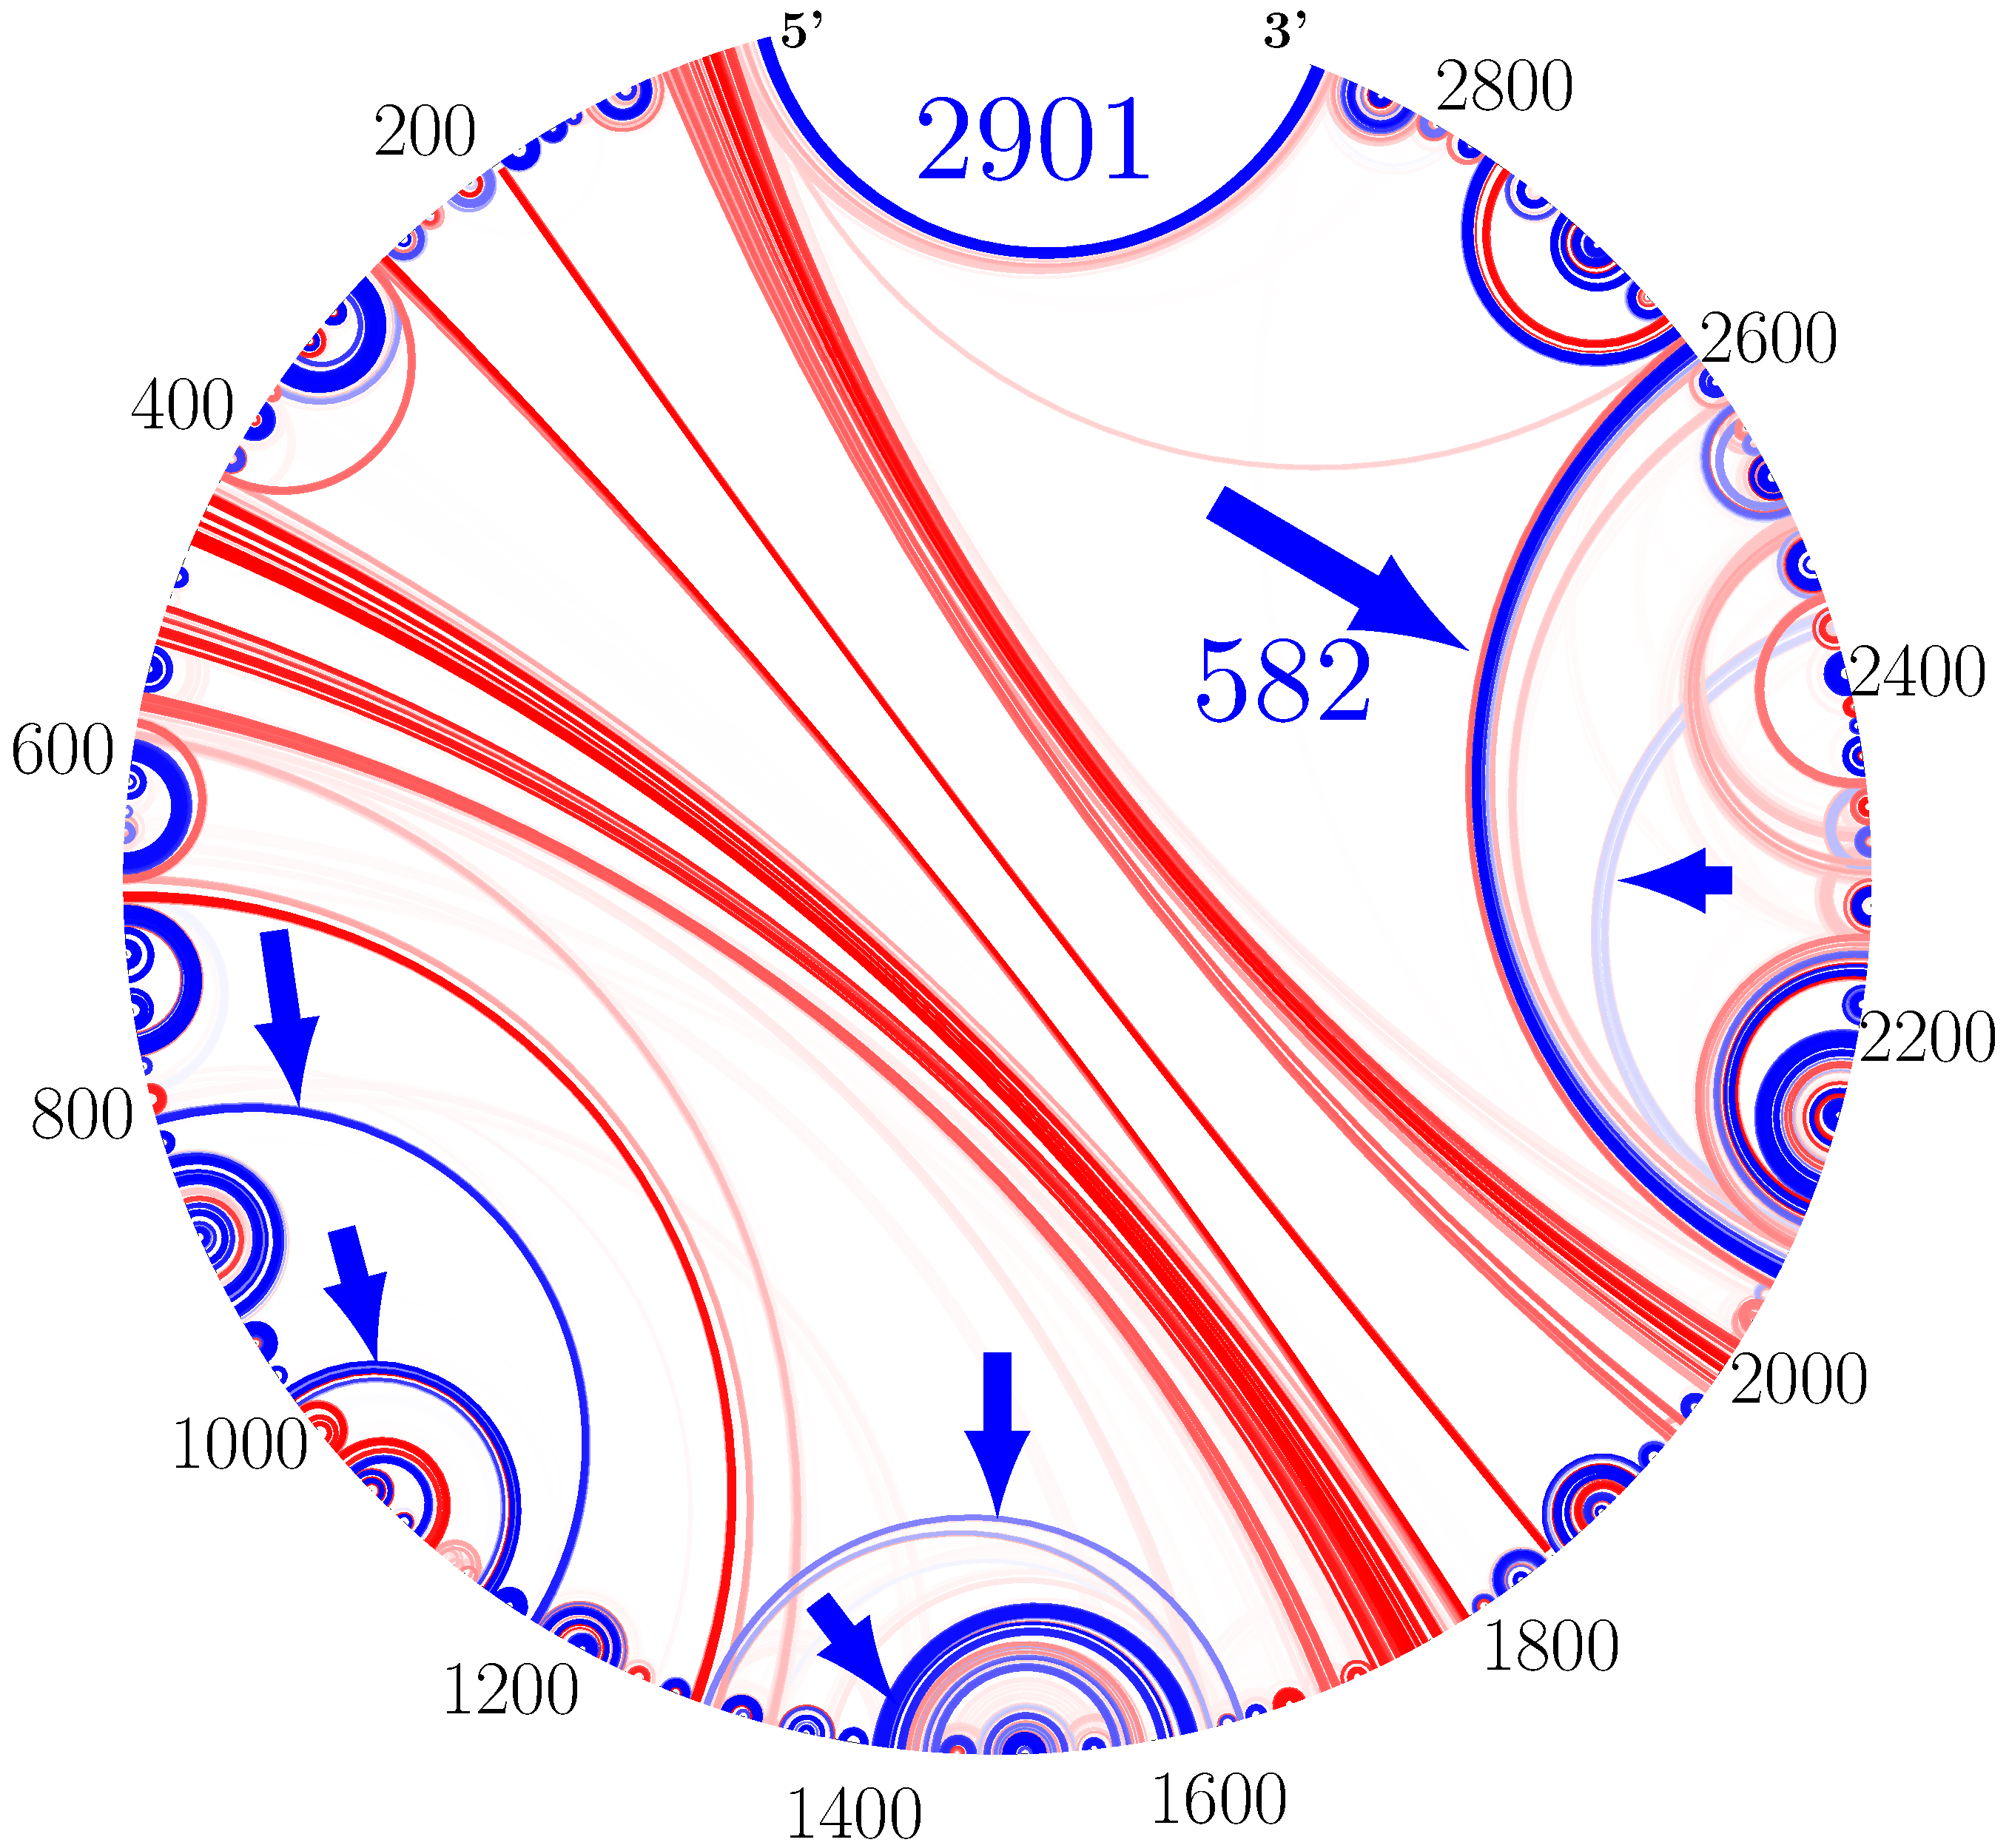
\includegraphics[width=0.25\textwidth]{figs/23s_example}} \\[-2.3cm]
% % } & \\[-.4cm]
% \hspace{-.2cm}\raisebox{1cm}{\panel{C}} & \\[-2.2cm]
% \hspace{-7cm}\panel{E} &\\[-.5cm]
% \multicolumn{2}{l}{% \hspace{-0.3cm}

\resizebox{0.5\textwidth}{!}
{
  \begin{tabular}{c}
%	\toprule
         % &     \multicolumn{2}{c}{total} & \multicolumn{2}{c}{correct} \\
			 % \midrule
\hspace{6.5cm}{\color{blue} $p_\linear \!-\! p_\vienna \!>\! 0.2$} \\[.3cm]
\hspace{6.4cm}{\color{darkgreen} $|p_\linear \!-\! p_\vienna| \!\leq \!0.2$} \\[.3cm]
\hspace{6.3cm}{\color{red} $p_\linear \!-\! p_\vienna \!<\! -0.2$}  \\[-2.4cm]
%	                 \bottomrule
  \end{tabular}
 }

% \resizebox{0.45\textwidth}{!}
% \panel{C}}
\vspace{.5cm}
{
  \hspace{-4.5cm}\begin{tabular}{r@{\; }r@{\quad}r@{\; }r}
%	\toprule
% \panel{C}} & &&\\
          \multicolumn{2}{c}{total} & \multicolumn{2}{c}{correct} \\
			 \midrule
55 \bluetri & 40 \bluecir  & 23 \bluetri & 37 \bluecir \\
  126,645 \greentri & 420 \greencir & 111 \greentri & 180 \greencir\\
 56 \redtri & 44 \redcir & 0 \redtri & 19 \redcir \\[1.9cm]
%	                 \bottomrule
  \end{tabular}
  }

% }
% &\\[-2cm]
% &\raisebox{5cm}{\hspace{-0.2cm}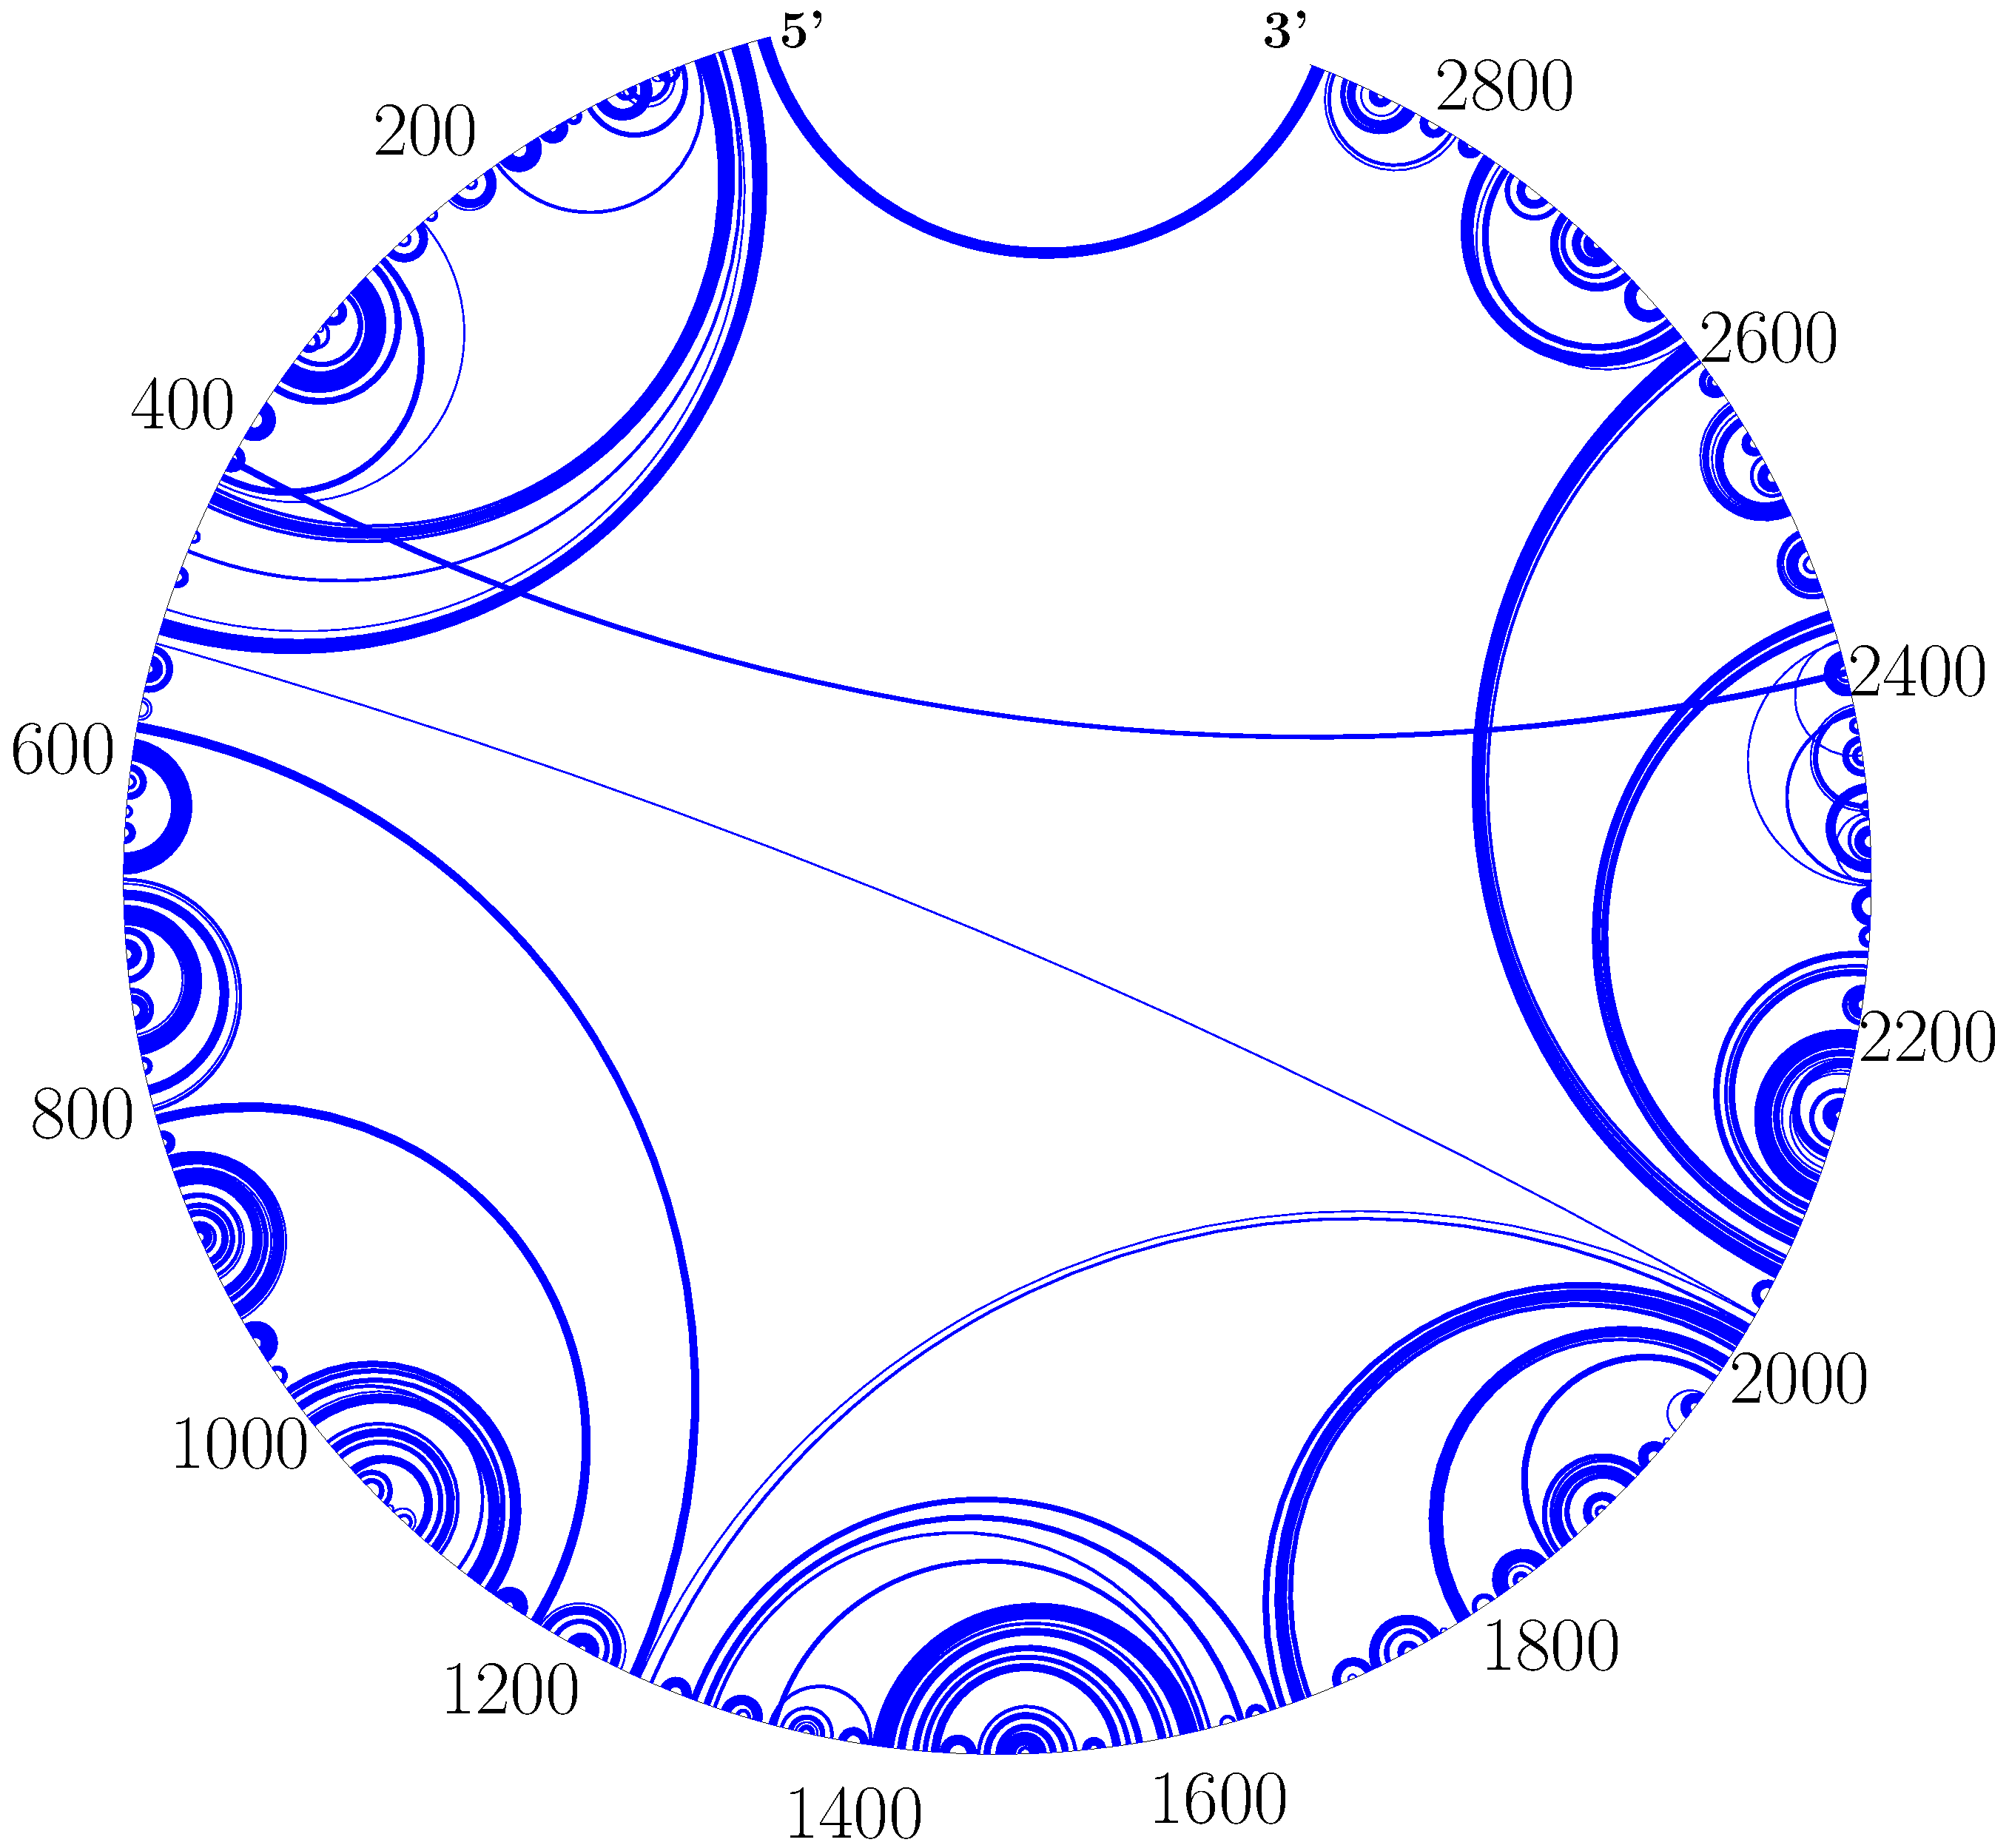
\includegraphics[width=0.25\textwidth]{figs/23s_gold}} \\
% \end{tabular}\\

% \begin{tabular}{cccc}
% \hspace{-4.4cm} \panel{F} & \hspace{-4.6cm}\panel{G} & \hspace{-4.6cm}\panel{H} & \hspace{-4.6cm}\panel{I}\\[-0.2cm]
% \hspace{-0.2cm}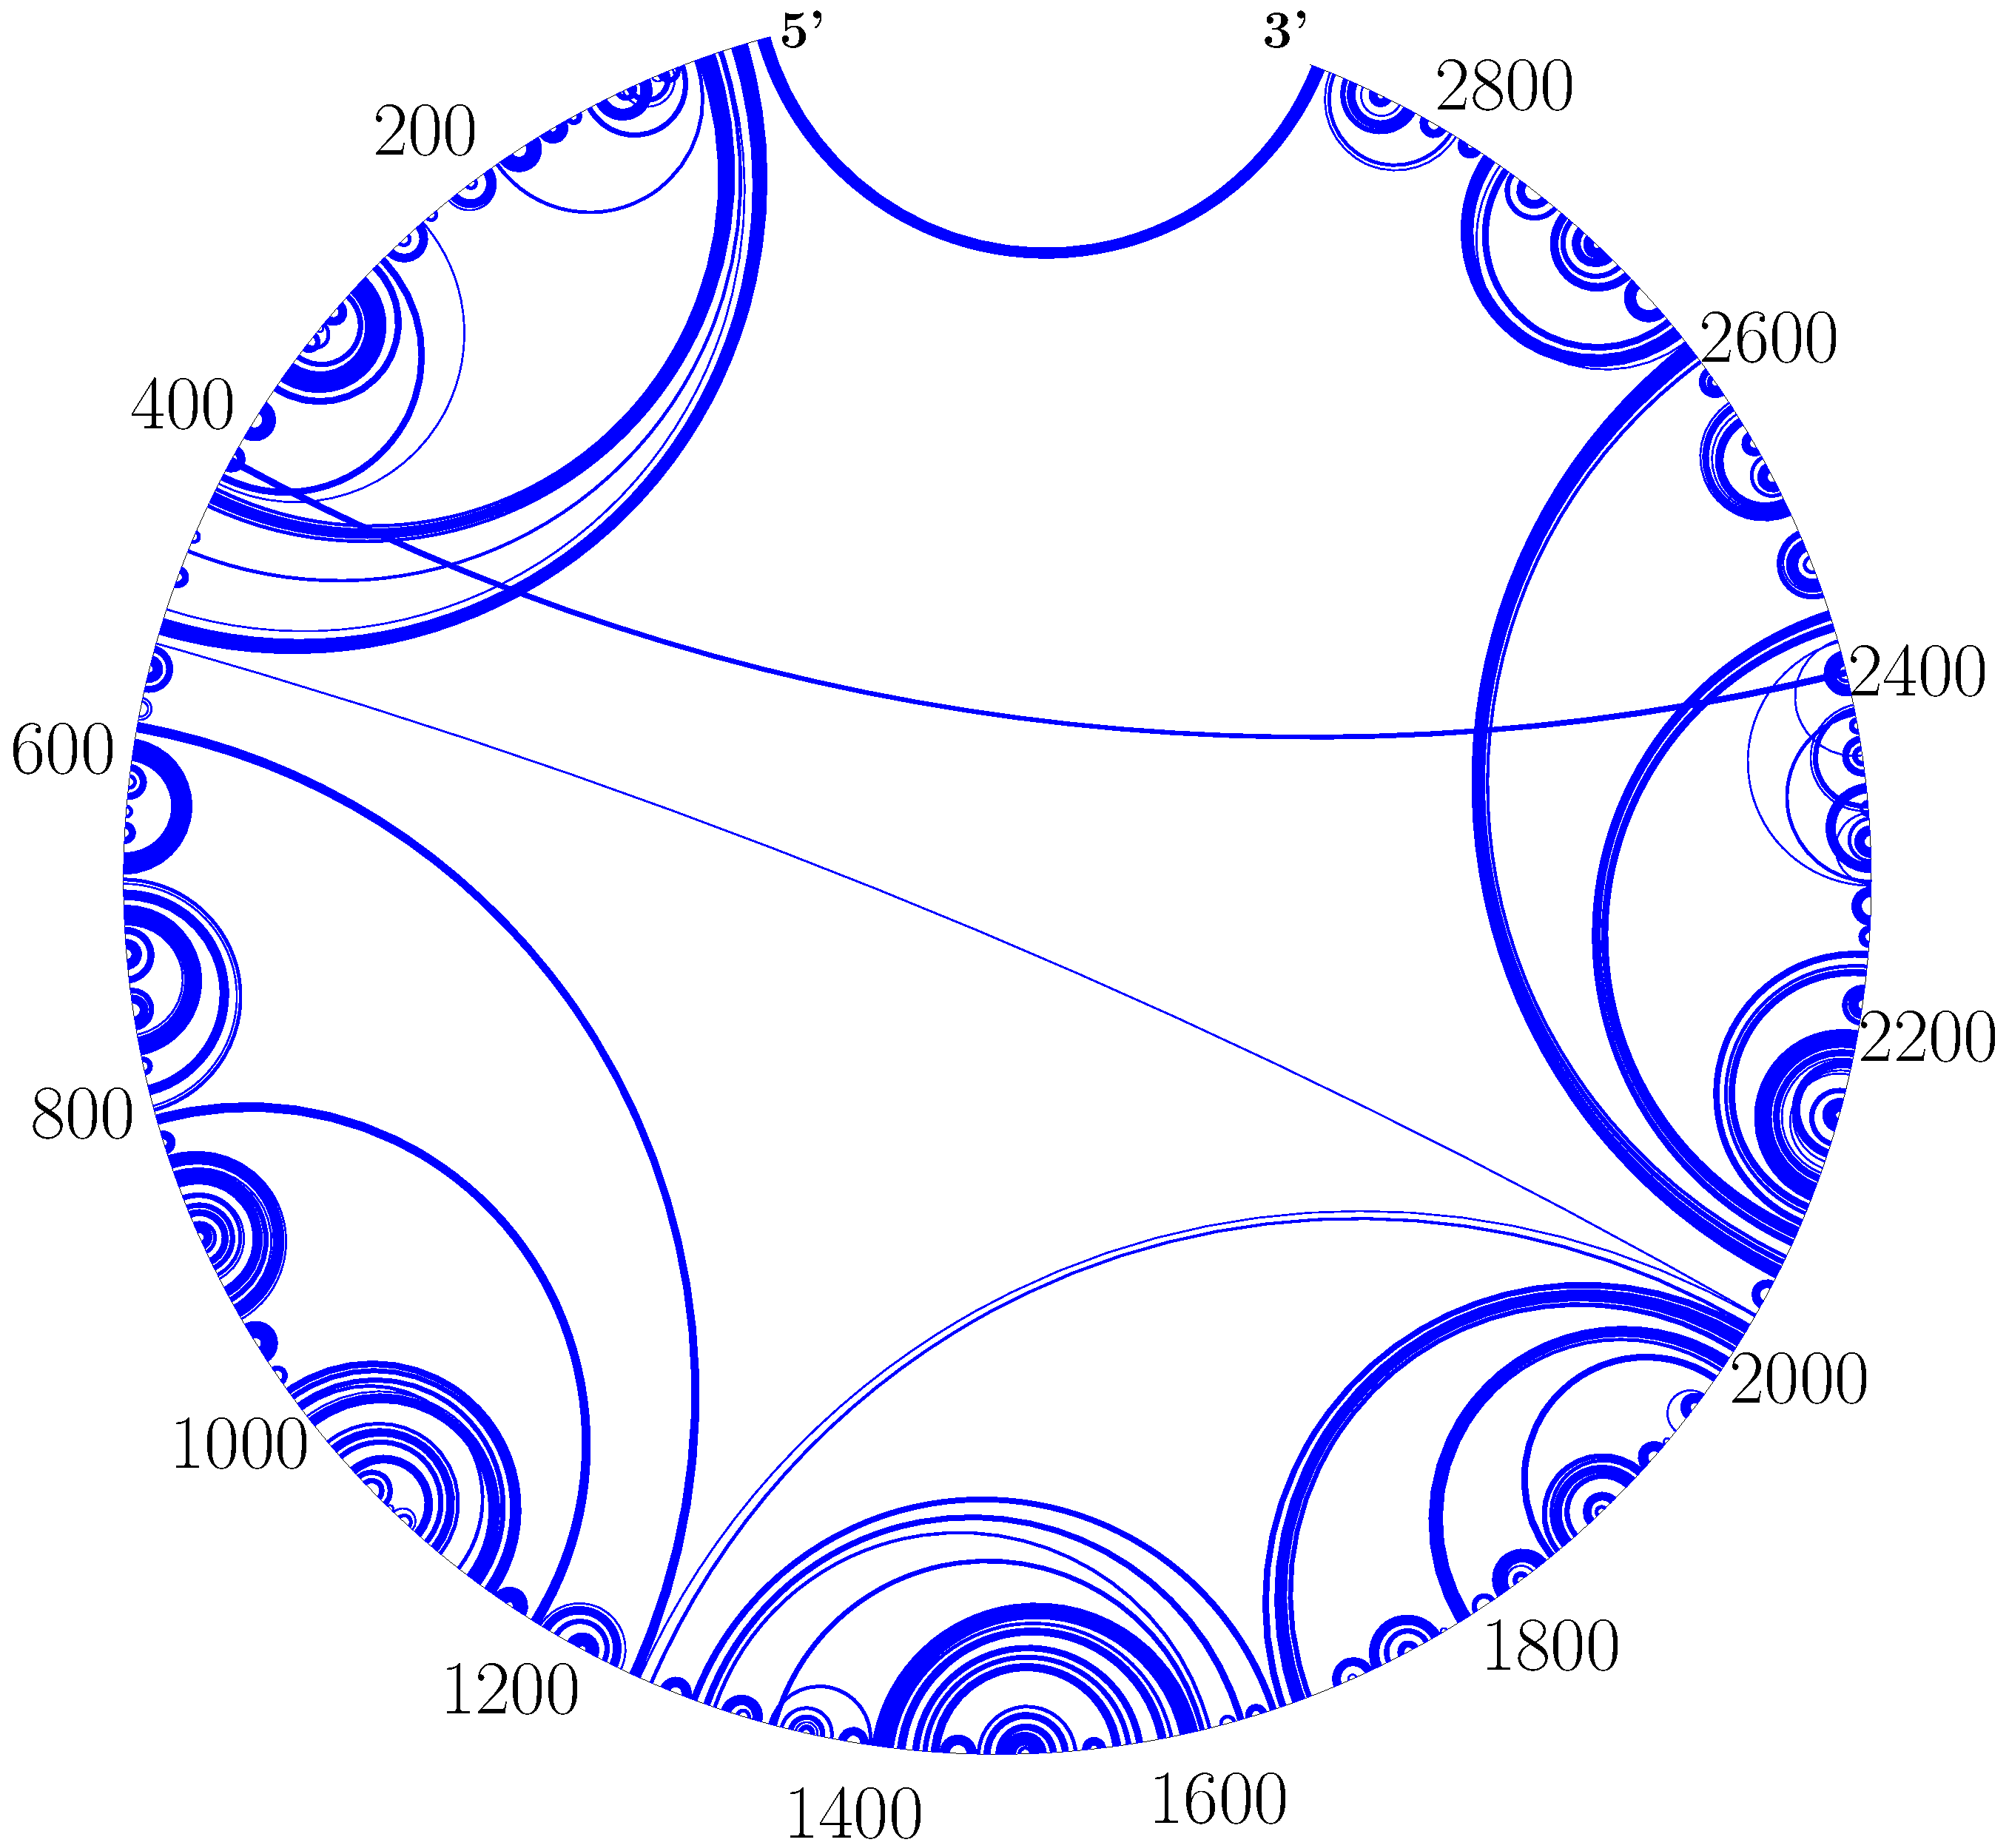
\includegraphics[width=0.25\textwidth]{figs/23s_gold} &
% \hspace{-0.35cm}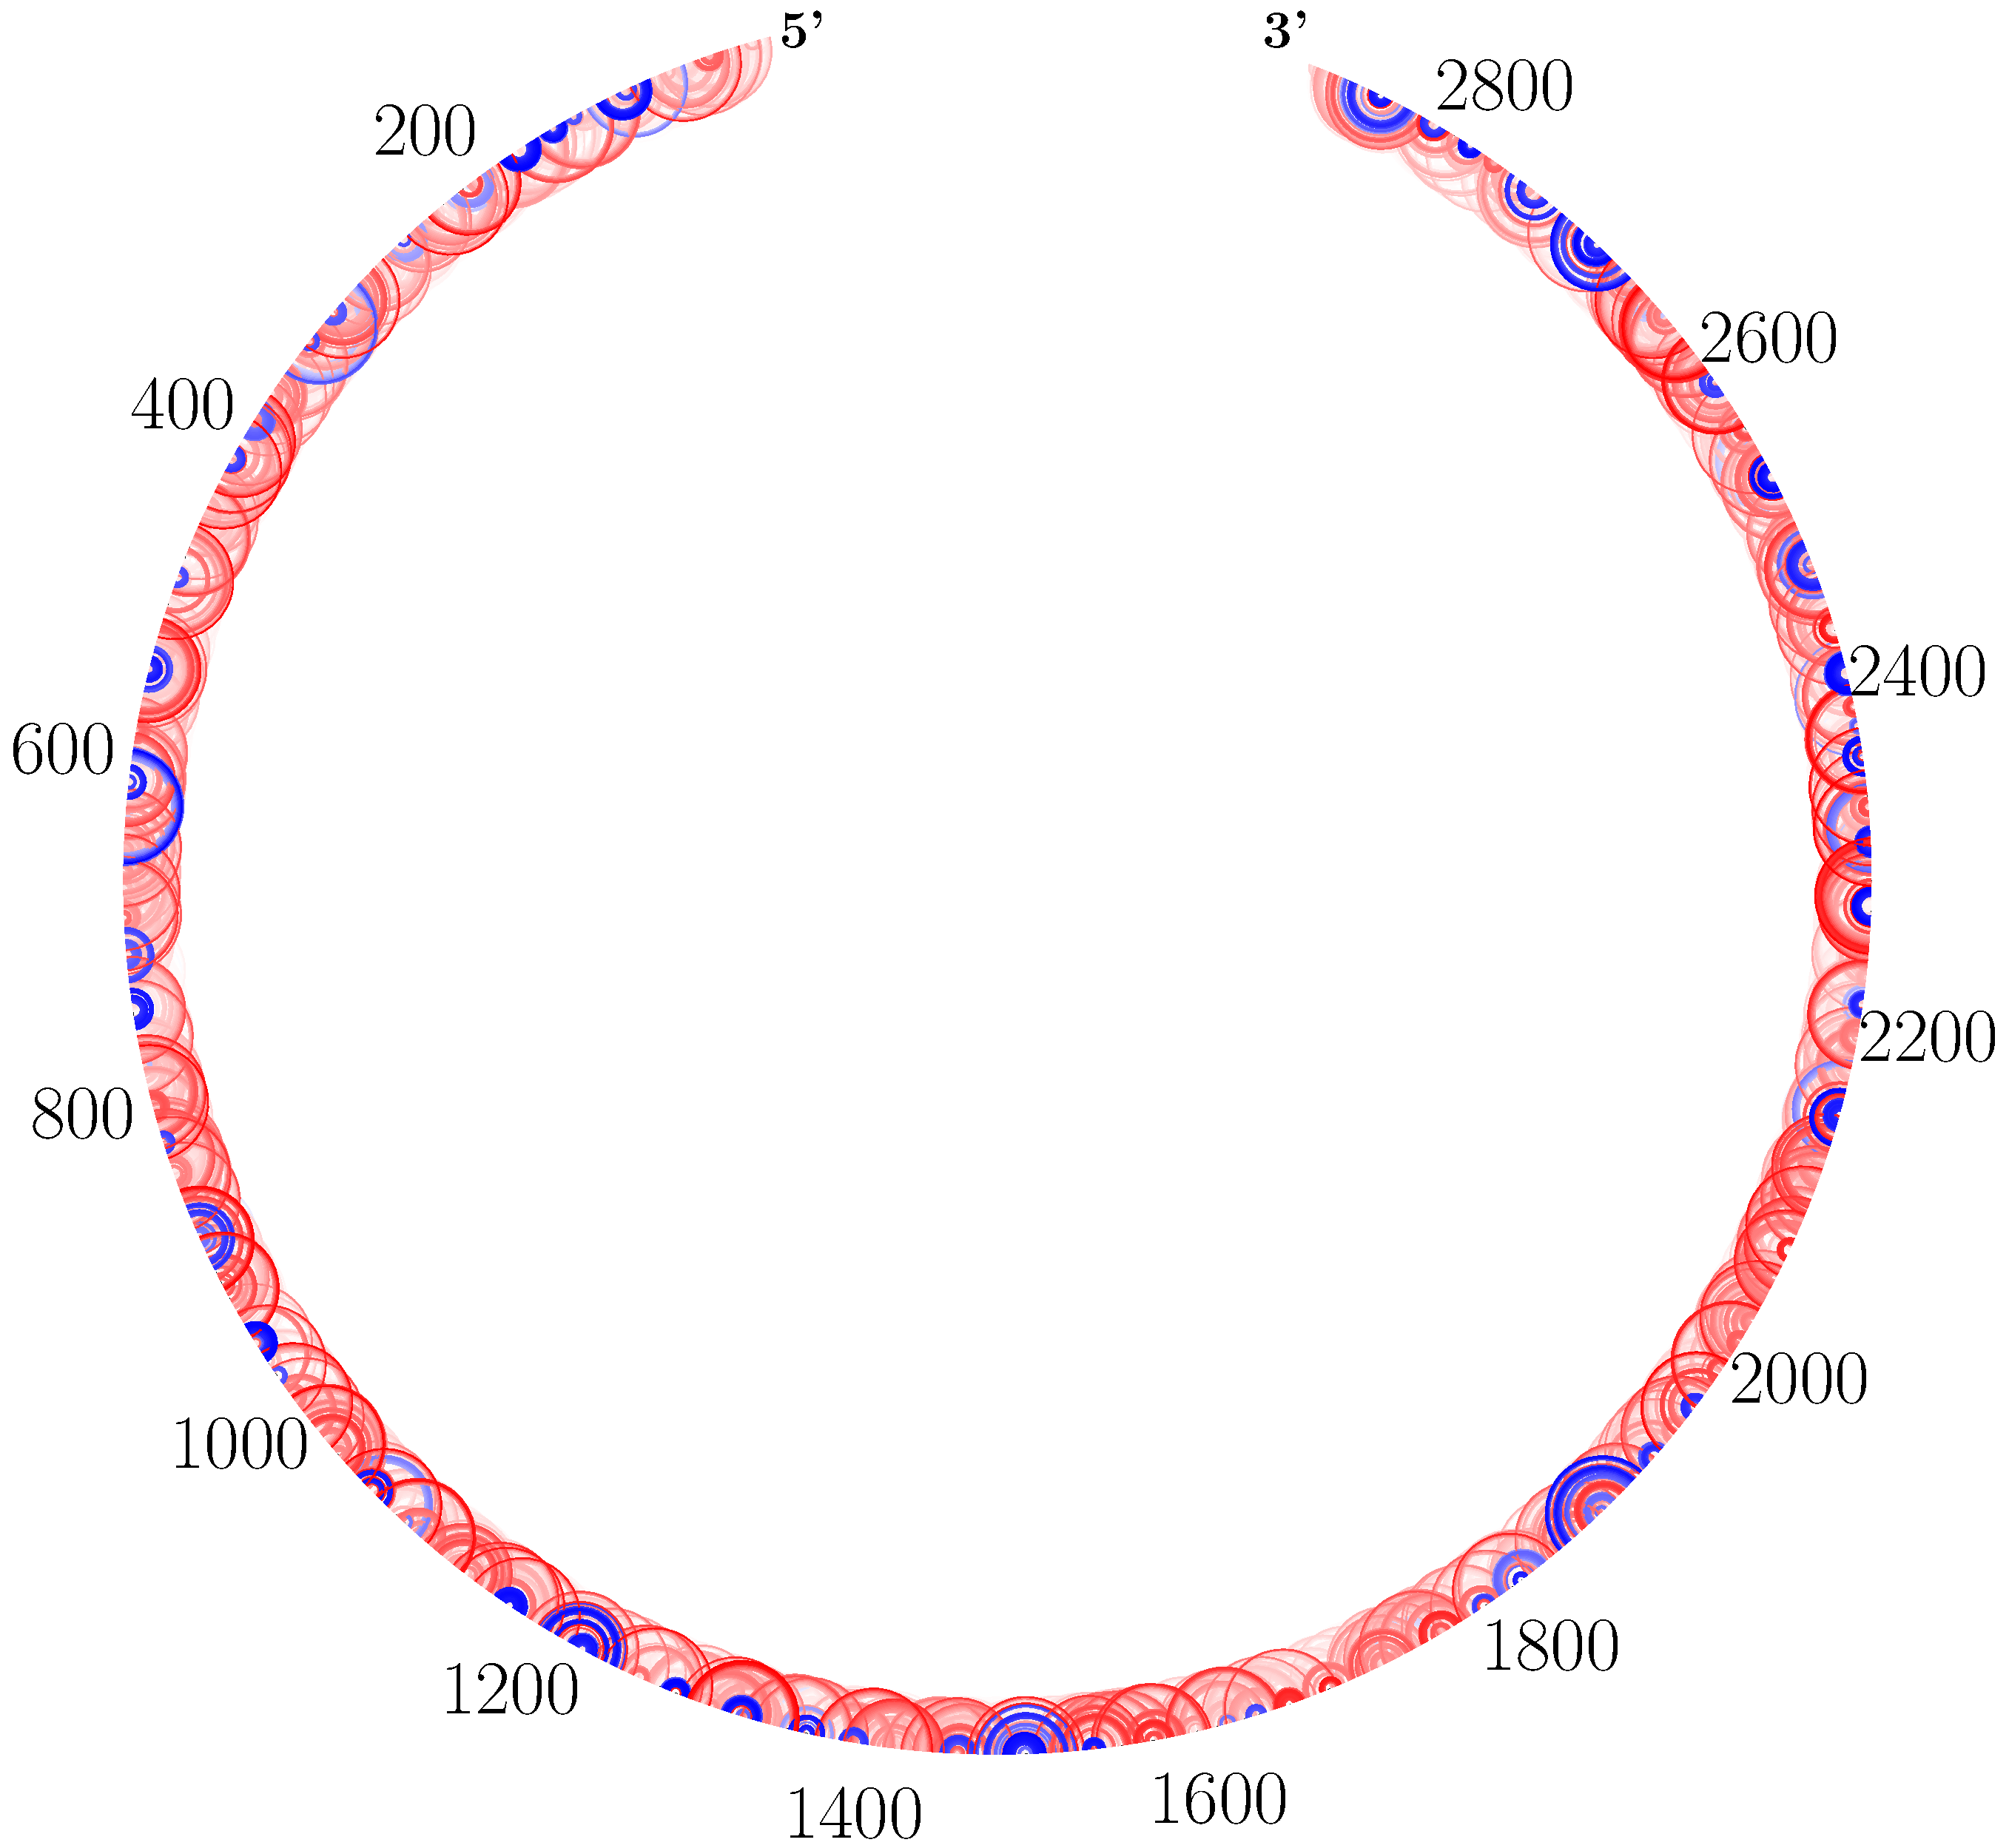
\includegraphics[width=0.25\textwidth]{figs/23s_vienna_plfold_example.pdf} &
% \hspace{-0.35cm}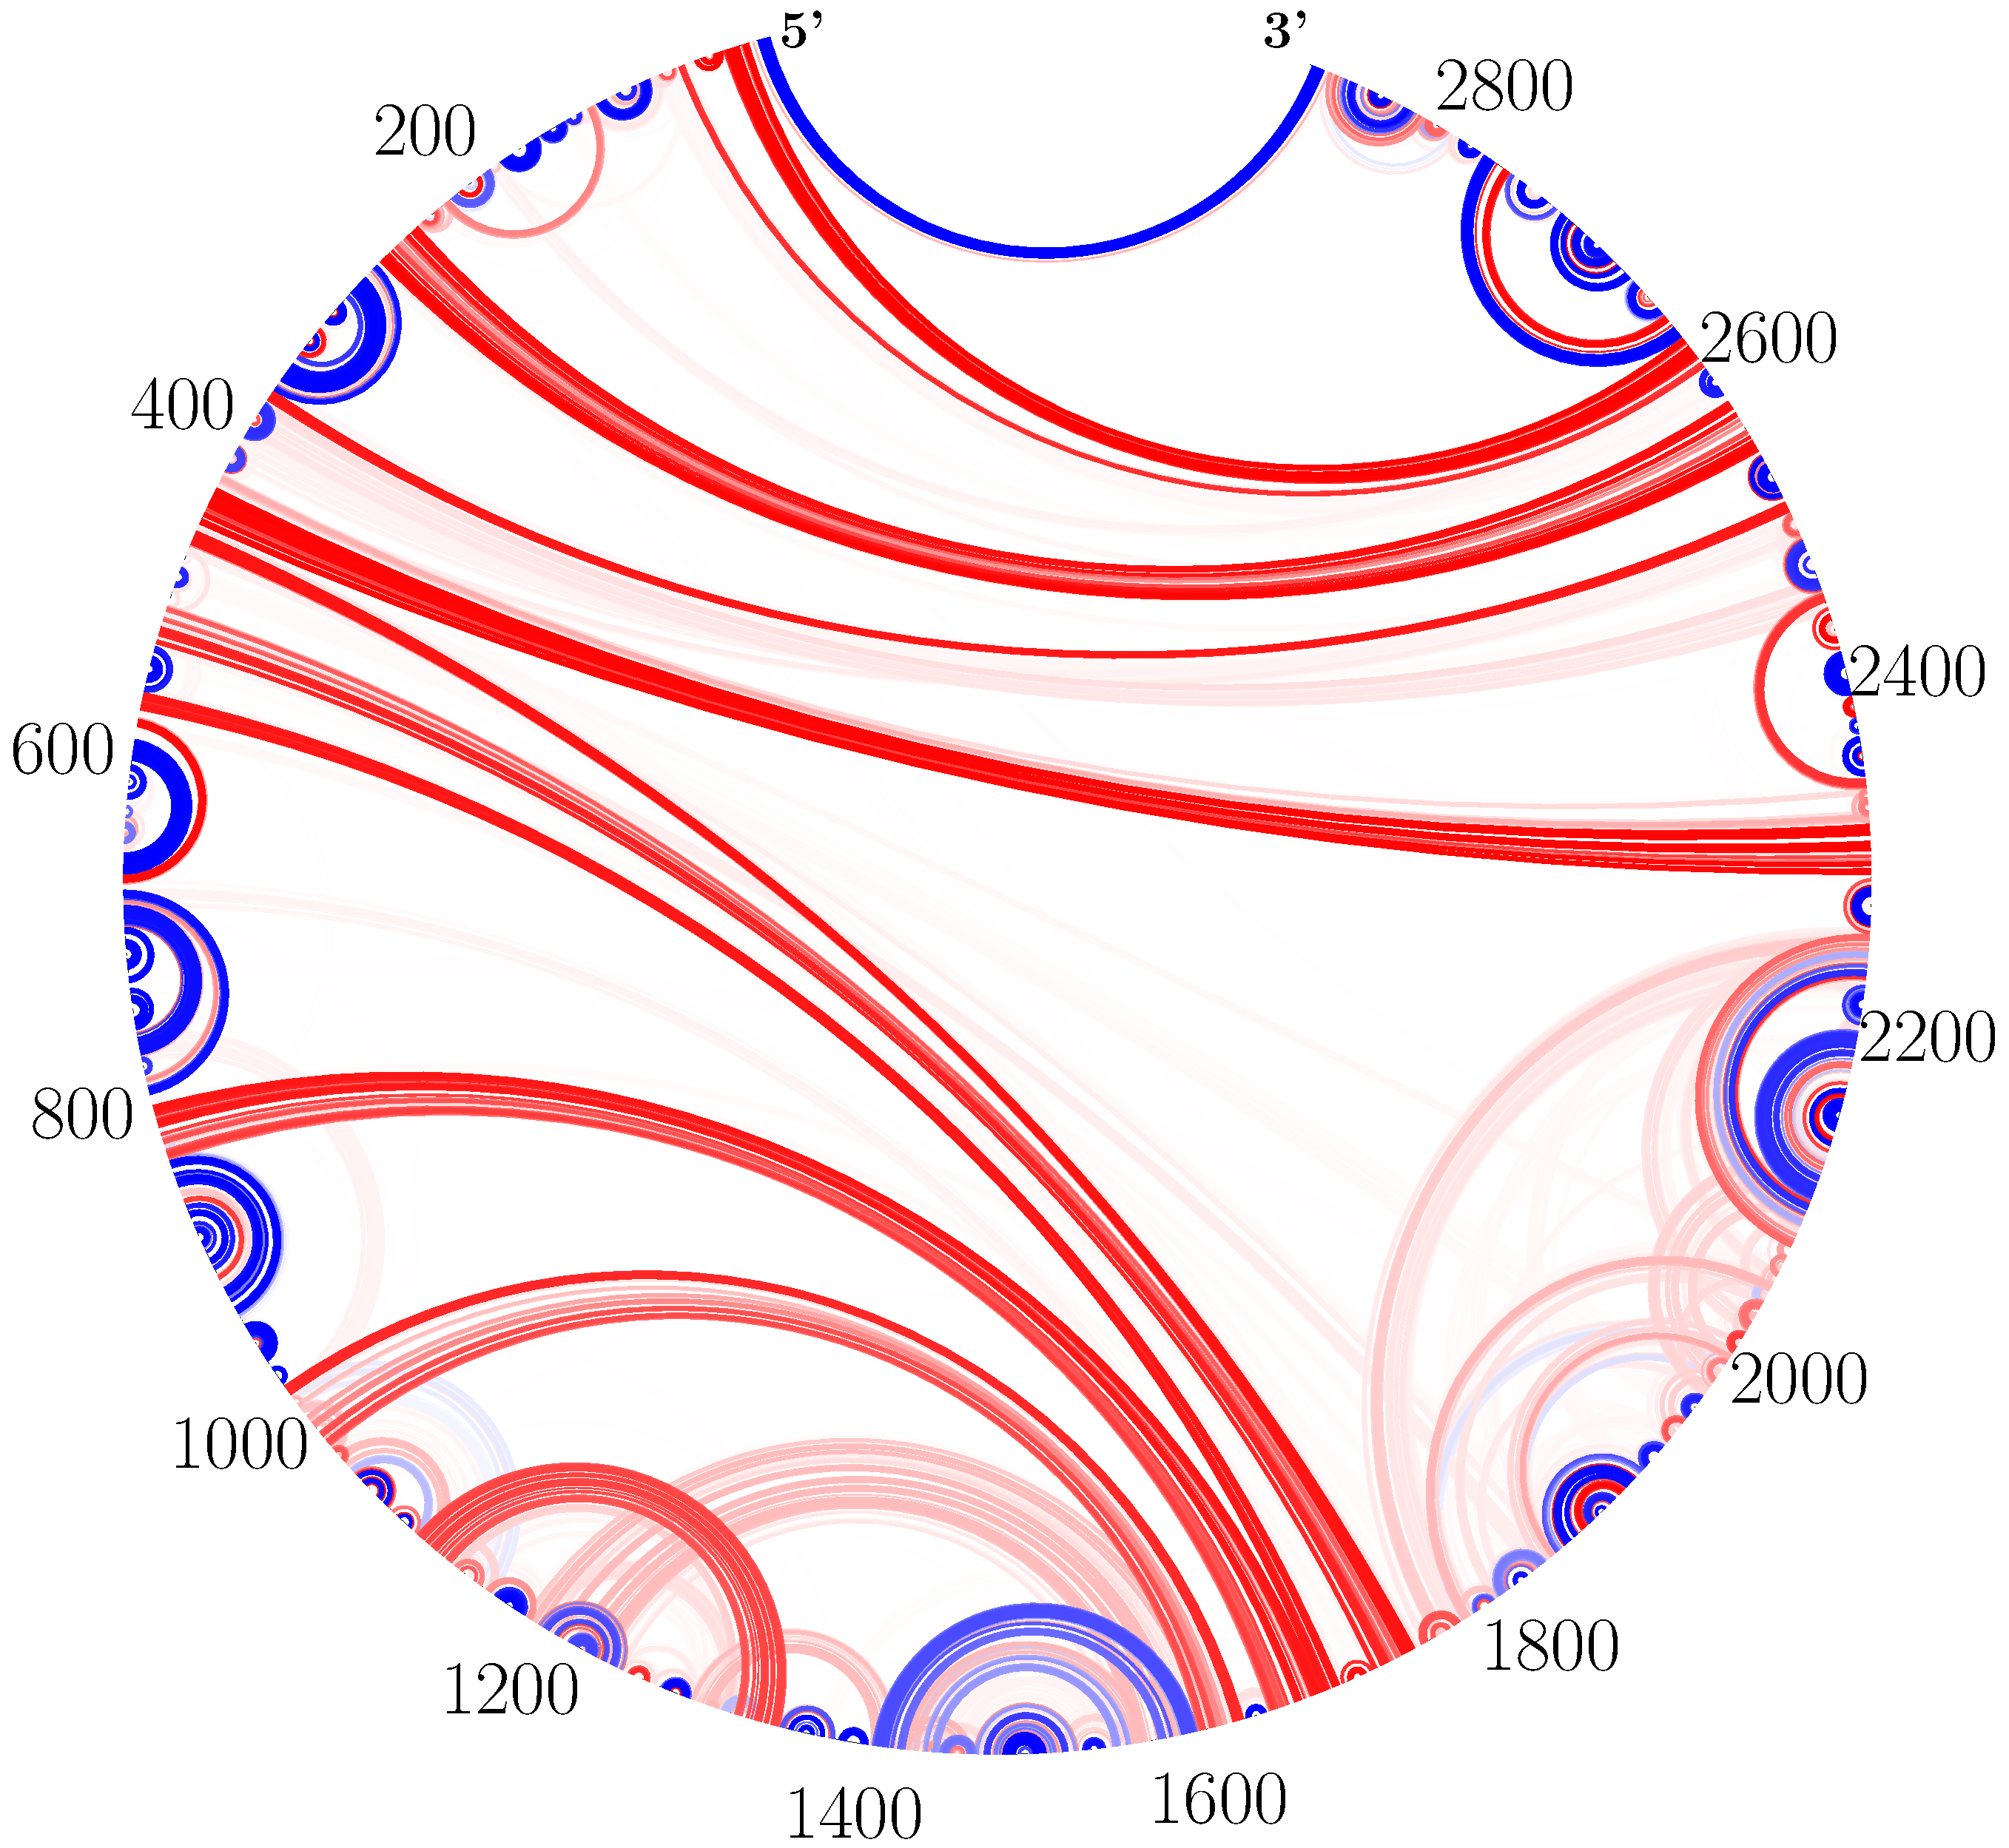
\includegraphics[width=0.25\textwidth]{figs/23s_vienna_example} &
% \hspace{-0.35cm}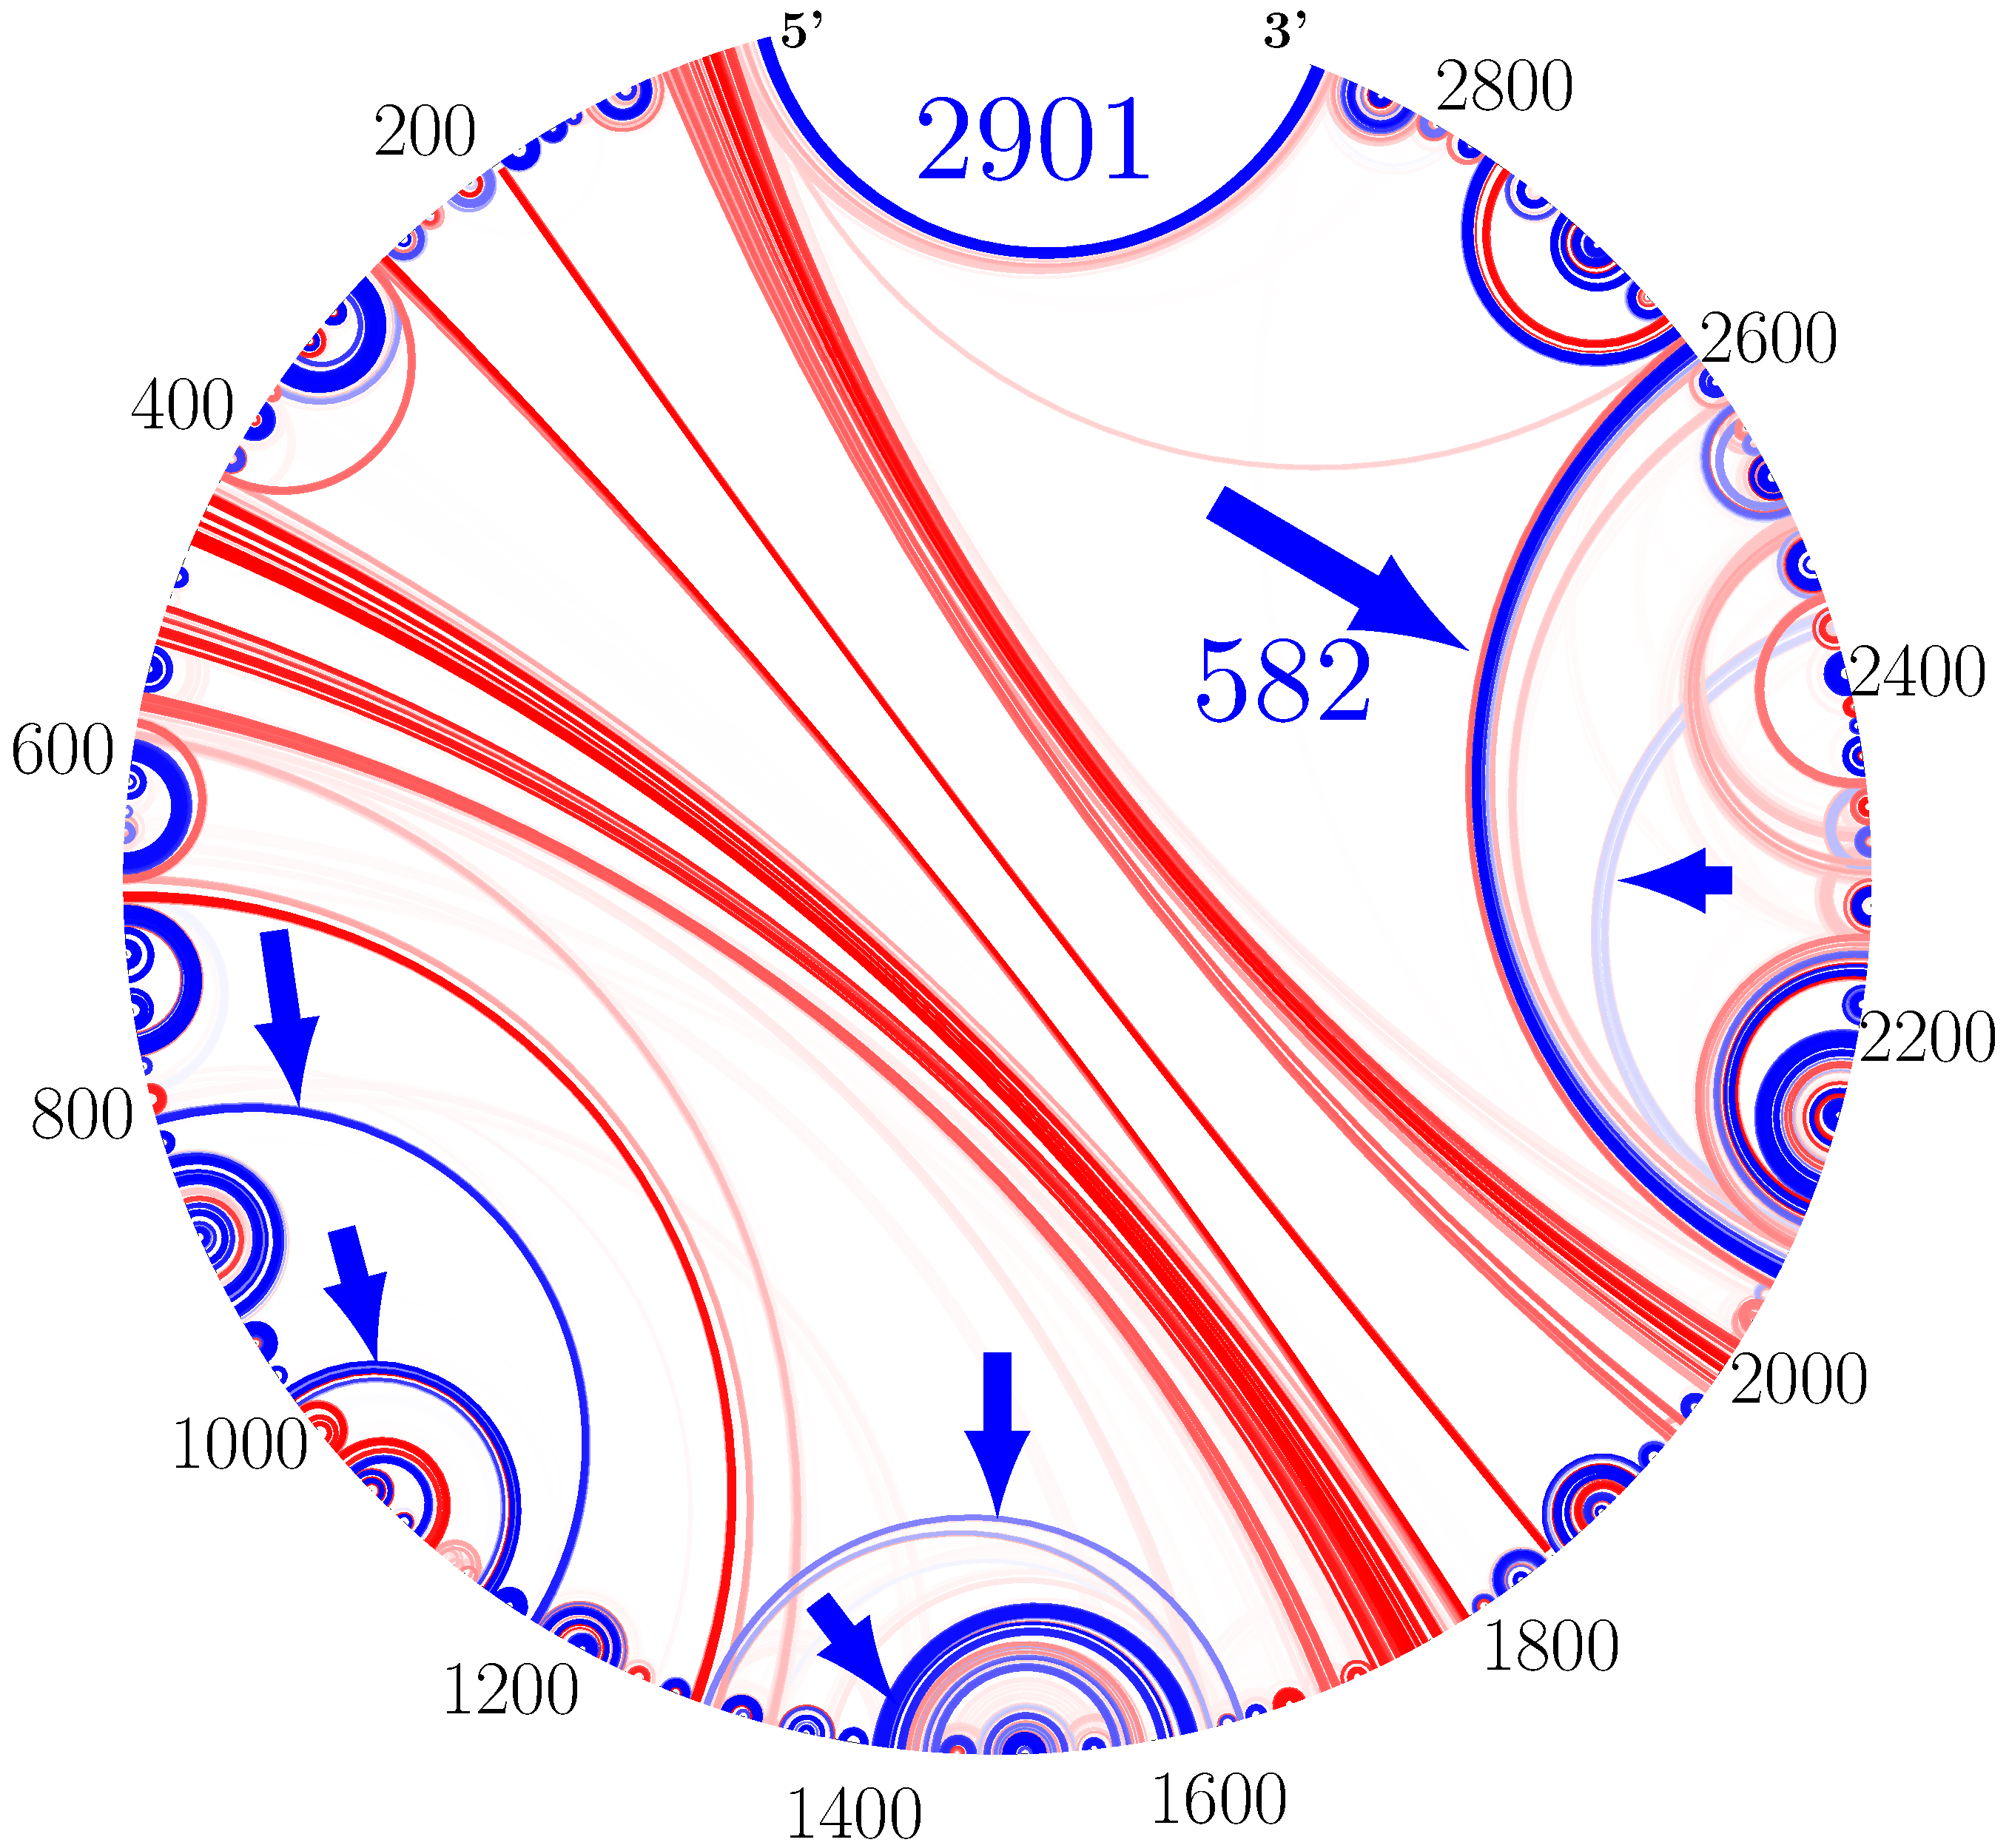
\includegraphics[width=0.25\textwidth]{figs/23s_example.pdf}
% \end{tabular}
\vspace{-2cm}
\caption{
{\bf A--C}: An example of {\it C.~ellipsoidea} Group I Intron. 
{\bf A}: Solid triangles ({\small {\color{blue} $\blacktriangle$} {\color{darkgreen}$\blacktriangle$}  {\color{red}$\blacktriangle$}}) stand for base pairing probabilities and
unfilled circles ({\small {\color{blue} $\circ$} {\color{darkgreen}$\circ$}  {\color{red}$\circ$}})  stand for single-stranded probabilities.
{\color{blue} blue: $p_\linear \!-\! p_\vienna \!>\! 0.2$};
{\color{darkgreen} green: $|p_\linear \!-\! p_\vienna| \!\leq \!0.2$};
{\color{red} red: $p_\linear \!-\! p_\vienna \!<\! -0.2$};
%some high probability pairs and unpaired bases in \linearpartition have low probabilities in \viennarnafold (in blue), and some low probability ones in \linearpartition have high probabilities in \viennarnafold (in red); 
	{\bf B}: Ground truth structure colored with the above scheme; % from \viennarnafold and \linearpartition; 
	%pink binds around position 370 are pseudoknotted pairs.
	{\bf C}: Statistics of this example. 
	"total" columns are the total numbers of triangles and circles with different colors in {\bf A},
	while "correct" columns are the corresponding numbers %of such triangles and circles
        in the ground-truth structure  in {\bf B},
        which is better correlated with \linearpartition's probabilities than \viennarnafold's ({\color{blue} 23 blue pairs} and {\color{red} 0 red pairs}). %ground-truth structure.
	% Note that each triangle represents a pair of nucleotides.
%% {\bf D--G}: An example of \ecoli 23S rRNA. 
%% 	{\bf D}: circular plot of the ground truth.
%% {\bf E--G}: circular plots using the base pair probabilities from \viennarnaplfold (with default window size $70$), \rnafold and \linearpartition, respectively; 
%% base pairs in the ground truth are in blue;
%% the color shade of the lines are propotional to their probabilities.
	\label{fig:example}\\[-.7cm]
}
\end{figure}
